% Seminarul 11: Ipoteza piețelor fractale și memoria lungă
% Statistica piețelor financiare -- Program de licență, Academia de Studii Economice din București
% GENERAT de latex/build_seminar11.py -- modificați generatorul, nu acest fișier.
% Implicit versiunea pentru studenți; versiunea profesorului este wrapper-ul *_solutions.tex.
\makeatletter\@ifundefined{ifsolutions}{\expandafter\newif\csname ifsolutions\endcsname}{}\makeatother

\newcommand{\coursename}{Statistica piețelor financiare}
\def\sfmlang{ro}
% Preambul comun SFM -- Statistica piețelor financiare / Statistics of Financial Markets (Beamer, 16:9)
% Același design ca MFM. Înainte de % Preambul comun SFM -- Statistica piețelor financiare / Statistics of Financial Markets (Beamer, 16:9)
% Același design ca MFM. Înainte de % Preambul comun SFM -- Statistica piețelor financiare / Statistics of Financial Markets (Beamer, 16:9)
% Același design ca MFM. Înainte de \input{../../latex/preamble} se definește
%   \newcommand{\coursename}{Statistics of Financial Markets}      (EN)
%   \newcommand{\coursename}{Statistica piețelor financiare}       (RO)  și  \def\sfmlang{ro}
% Fișierele .tex se află în EN/Courses, EN/Seminars, RO/Cursuri, RO/Seminarii (două niveluri sub rădăcină).
% Deck-urile sînt generate de latex/build_chapterN.py / build_seminarN.py (vezi latex/sfm_build.py).

\documentclass[9pt, aspectratio=169, t]{beamer}
\providecommand{\coursename}{Statistics of Financial Markets}

% Ensure content fits on slides
\setbeamersize{text margin left=8mm, text margin right=8mm}

%=============================================================================
% THEME AND STYLE CONFIGURATION
%=============================================================================
\usetheme{default}
% Using default theme for clean header/footer control

% Color Palette (matching Redispatch PDF)
\definecolor{MainBlue}{RGB}{26, 58, 110}
\definecolor{AccentBlue}{RGB}{26, 58, 110}
\definecolor{IDAred}{RGB}{205, 0, 0}
\definecolor{DarkGray}{RGB}{51, 51, 51}
\definecolor{MediumGray}{RGB}{128, 128, 128}
\definecolor{LightGray}{RGB}{248, 248, 248}
\definecolor{VeryLightGray}{RGB}{235, 235, 235}
\definecolor{KeynoteGray}{RGB}{218, 218, 218}
\definecolor{SectionGray}{RGB}{120, 120, 120}
\definecolor{FooterGray}{RGB}{100, 100, 100}
\definecolor{Crimson}{RGB}{220, 53, 69}
\definecolor{Forest}{RGB}{46, 125, 50}
\definecolor{Amber}{RGB}{181, 133, 63}
\definecolor{Orange}{RGB}{230, 126, 34}
\definecolor{Purple}{RGB}{142, 68, 173}

% Gradient background (exact Keynote 315° gradient: white to RGB 218,218,218)
\setbeamertemplate{background}{%
    \begin{tikzpicture}[remember picture, overlay]
        \shade[shading=axis, shading angle=315,
        top color=white, bottom color=KeynoteGray]
        (current page.south west) rectangle (current page.north east);
    \end{tikzpicture}%
}
% Fallback solid color for compatibility
\setbeamercolor{background canvas}{bg=}

\setbeamercolor{palette primary}{bg=MainBlue, fg=white}
\setbeamercolor{palette secondary}{bg=MainBlue!85, fg=white}
\setbeamercolor{palette tertiary}{bg=MainBlue!70, fg=white}
\setbeamercolor{structure}{fg=MainBlue}
\setbeamercolor{title}{fg=IDAred}
\setbeamercolor{frametitle}{fg=IDAred, bg=}
\setbeamercolor{block title}{bg=MainBlue, fg=white}
\setbeamercolor{block body}{bg=VeryLightGray, fg=DarkGray}
\setbeamercolor{block title alerted}{bg=Crimson, fg=white}
\setbeamercolor{block body alerted}{bg=Crimson!8, fg=DarkGray}
\setbeamercolor{block title example}{bg=Forest, fg=white}
\setbeamercolor{block body example}{bg=Forest!8, fg=DarkGray}
\setbeamercolor{item}{fg=MainBlue}

% Footer colors (override Madrid theme blue)
\setbeamercolor{author in head/foot}{fg=FooterGray, bg=}
\setbeamercolor{title in head/foot}{fg=FooterGray, bg=}
\setbeamercolor{date in head/foot}{fg=FooterGray, bg=}
\setbeamercolor{section in head/foot}{fg=FooterGray, bg=}
\setbeamercolor{subsection in head/foot}{fg=FooterGray, bg=}

% Bullet styles (apply everywhere including blocks)
\setbeamertemplate{itemize item}{\color{MainBlue}$\boxdot$}
\setbeamertemplate{itemize subitem}{\color{MainBlue}$\blacktriangleright$}
\setbeamertemplate{itemize subsubitem}{\color{MainBlue}\tiny$\bullet$}
\setbeamertemplate{itemize/enumerate body begin}{\normalsize}
\setbeamertemplate{itemize/enumerate subbody begin}{\normalsize}

% Item spacing - compact style
\setlength{\leftmargini}{10pt}       % Level 1: minimal indent
\setlength{\leftmarginii}{10pt}      % Level 2: minimal additional indent
% Compact list spacing (zero extra space before/after lists in blocks)
\makeatletter
\def\@listi{\leftmargin\leftmargini \topsep 0pt \parsep 0pt \itemsep 0pt}
\def\@listii{\leftmargin\leftmarginii \topsep 0pt \parsep 0pt \itemsep 0pt}
\makeatother

\setbeamertemplate{navigation symbols}{}

%=============================================================================
% CUSTOM HEADLINE
%=============================================================================
\setbeamertemplate{headline}{%
    \vskip10pt%
    \hbox to \paperwidth{%
        \hskip0.5cm%
        {\small\color{FooterGray}\renewcommand{\hyperlink}[2]{##2}\insertsectionhead}%
        \hfill%
        \textcolor{FooterGray}{\small\insertframenumber}%
        \hskip0.5cm%
    }%
    \vskip4pt%
    {\color{FooterGray}\hrule height 0.4pt}%
}

%=============================================================================
% CUSTOM FOOTER
%=============================================================================
\usepackage{fontawesome5}

\setbeamertemplate{footline}{%
    {\color{FooterGray}\hrule height 0.4pt}%
    \vskip4pt%
    \hbox to \paperwidth{%
        \hskip0.5cm%
        \textcolor{FooterGray}{\small\coursename}%
        \hfill%
        \raisebox{-0.1em}{%
            \begin{tikzpicture}[x=0.08em, y=0.08em, line width=0.4pt]
                \draw[FooterGray] (0,3) -- (1,4) -- (2,3.5) -- (3,5) -- (4,4) -- (5,6) -- (6,5.5) -- (7,4) -- (8,5) -- (9,7) -- (10,6) -- (11,5) -- (12,6.5) -- (13,8) -- (14,7) -- (15,6) -- (16,7.5) -- (17,9) -- (18,8) -- (19,7) -- (20,8.5) -- (21,10) -- (22,9) -- (23,8) -- (24,9.5);
            \end{tikzpicture}%
        }%
        \hskip0.5cm%
    }%
    \vskip6pt%
}

%=============================================================================
% PACKAGES
%=============================================================================
\usepackage[utf8]{inputenc}
\DeclareUnicodeCharacter{03B1}{\ensuremath{\alpha}}
\usepackage[T1]{fontenc}
\usepackage{amsmath, amssymb, amsthm}
\usepackage{mathtools}
\usepackage{bm}
\usepackage{tikz}
\usetikzlibrary{arrows.meta, positioning, shapes, calc, decorations.pathreplacing, shadings}
\usepackage{booktabs}
\usepackage{multirow}
\usepackage{array}
\usepackage{graphicx}
\usepackage{hyperref}
\usepackage{colortbl}
\usepackage{listings}
\lstset{language=Python, basicstyle=\ttfamily\scriptsize, keywordstyle=\color{MainBlue}\bfseries,
  commentstyle=\color{Forest}, stringstyle=\color{Crimson}, breaklines=true,
  frame=none, backgroundcolor=\color{VeryLightGray}, xleftmargin=2mm}
\hypersetup{colorlinks=true, linkcolor=MainBlue, urlcolor=MainBlue}
\graphicspath{{../../logos/}{../../charts/}{../../photos/}}
\usepackage{xcolor}
\hfuzz=2pt  % Suppress tiny overfull warnings (<2pt)
\vfuzz=2pt  % Suppress tiny vertical overfull warnings (<2pt)

%=============================================================================
% QUANTLET COMMANDS
%   \quantlet{<displayed name>}{<url>}       (generic, compatible with the older SFM decks)
%   \sfmquantlet{Ch_05}{SFM_ch5_garch}       -> https://github.com/danpele/SFM/tree/main/Quantlets/Ch_05/SFM_ch5_garch
%   \qlurl{<folder>} is defined per chapter by the generator (Quantlets/Ch_NN/<folder>)
%=============================================================================
\newcommand{\sfmrepo}{https://github.com/danpele/SFM}
\newcommand{\sfmqlbase}{https://github.com/danpele/SFM/tree/main/Quantlets}
\newcommand{\quantlet}[2]{%
    \hfill\href{#2}{%
        \raisebox{-0.15em}{
\includegraphics[height=0.7em]{ql_logo.png}}%
        \textcolor{MainBlue}{\tiny\ #1}%
    }%
}
\newcommand{\sfmquantlet}[2]{\quantlet{\detokenize{#2}}{\sfmqlbase/#1/#2}}

%=============================================================================
% NOTEBOOKS (Google Colab)
%   \colaburl{notebooks/EN/chapter5_seminar_notebook.ipynb} -> the Colab link of a file in the SFM repo
%   \nb: the chapter notebook (each seminar deck redefines it with \renewcommand)
%=============================================================================
\newcommand{\colaburl}[1]{https://colab.research.google.com/github/danpele/SFM/blob/main/#1}
\newcommand{\nb}{https://colab.research.google.com/github/danpele/SFM/tree/main/notebooks/EN}
\newcommand{\nbname}{notebooks/EN}

%=============================================================================
% SLIDE HELPERS (used by the generators; the same as in MFM)
%=============================================================================
% local font size for list bodies (the preamble forces \normalsize)
\newcommand{\itemsize}[1]{\setbeamertemplate{itemize/enumerate body begin}{#1}\setbeamertemplate{itemize/enumerate subbody begin}{#1}}
\newcommand{\intitle}[1]{{\hypersetup{urlcolor=white}#1}}   % white links inside coloured title bars
\newcommand{\imgcap}[1]{{\scriptsize #1}\\[0.5mm]}          % caption under a photo
\newcommand{\imgcredit}[2]{{\tiny\color{FooterGray}\href{#1}{#2}}}   % image credit: source URL, author/licence
\newcommand{\aiprompt}[1]{{\ttfamily\color{MainBlue}#1}}     % a prompt to an AI assistant

%=============================================================================
% SEMINARS: student version by default; the instructor wrapper *_solutions.tex sets \solutionstrue
%=============================================================================
\makeatletter\@ifundefined{ifsolutions}{\expandafter\newif\csname ifsolutions\endcsname}{}\makeatother
\newcommand{\solonly}[1]{\ifsolutions #1\fi}
\newcommand{\propsub}{\ifsolutions\else\framesubtitle{\ifdefined\sfmlang Rezolvarea se discută la seminar\else Solution discussed in class\fi}\fi}

%=============================================================================
% APPENDIX AND CHAPTER LINKS (latex/appendix_links.py writes the calls; it also re-declares these
% macros before \begin{document}, so the decks compile with or without this preamble block)
%=============================================================================
\providecommand{\sfmapplink}[3]{\hypertarget{#2}{}\hyperlink{#1}{\beamergotobutton{#3}}}
\providecommand{\sfmappback}[2]{\begin{tikzpicture}[remember picture,overlay]\node[anchor=south east] at ([xshift=-3mm,yshift=7mm]current page.south east){\hyperlink{#1}{\beamerreturnbutton{#2}}};\end{tikzpicture}}
\providecommand{\sfmchlink}[2]{\href{#1}{#2}}
\providecommand{\sfmchlinkt}[2]{\href{#1}{\usebeamercolor[fg]{frametitle}#2}}

%=============================================================================
% QUANTINAR COMMAND: link către un curs Quantinar (subiecte avansate)
%=============================================================================
\newcommand{\quantinar}[2]{%
    \href{#2}{%
        \raisebox{-0.15em}{
\includegraphics[height=0.8em]{qr_logo.png}}%
        \textcolor{MainBlue}{\scriptsize\ #1}%
    }%
}

%=============================================================================
% CUSTOM TITLE PAGE
%=============================================================================
\defbeamertemplate*{title page}{hybrid}[1][]
{
    \vspace{0.2cm}
    % Logos row - top header (with clickable links)
    \begin{center}
        \href{https://www.ase.ro}{
\includegraphics[height=1.0cm]{ase_logo.png}}\hspace{0.3cm}%
        \href{https://theida.net}{
\includegraphics[height=1.0cm]{ida_logo.png}}\hspace{0.3cm}%
        \href{https://blockchain-research-center.com}{
\includegraphics[height=1.0cm]{brc_logo.png}}\hspace{0.3cm}%
        \href{https://www.ai4efin.ase.ro}{
\includegraphics[height=1.0cm]{ai4efin_logo.png}}\hspace{0.3cm}%
        \href{https://ipe.ro/new}{
\includegraphics[height=1.0cm]{acad_logo.png}}\hspace{0.3cm}%
        \href{https://www.digital-finance-msca.com}{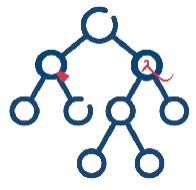
\includegraphics[height=1.0cm]{msca_logo.png}}%
    \end{center}

    \vspace{0.6cm}

    % Main title with Q logos on sides (with clickable links)
    \begin{center}
        \begin{minipage}{0.1\textwidth}
            \centering
            \href{https://quantlet.com}{
\includegraphics[height=1.1cm]{ql_logo.png}}
        \end{minipage}%
        \begin{minipage}{0.78\textwidth}
            \centering
            {\LARGE\bfseries\usebeamercolor[fg]{title}\inserttitle}

            \vspace{0.3cm}

            {\usebeamerfont{subtitle}\usebeamercolor[fg]{title}\insertsubtitle}
        \end{minipage}%
        \begin{minipage}{0.1\textwidth}
            \centering
            \href{https://quantinar.com}{
\includegraphics[height=1.1cm]{qr_logo.png}}
        \end{minipage}
    \end{center}

    \vspace{0.6cm}

    % Authors (left aligned)
    \hspace{0.5cm}{\usebeamerfont{author}\insertauthor}

    \vspace{0.3cm}

    % Institute/Affiliations (left aligned)
    \hspace{0.5cm}\begin{minipage}[t]{0.9\textwidth}
        \raggedright\small\insertinstitute
    \end{minipage}
}

%=============================================================================
% THEOREM ENVIRONMENTS
%=============================================================================
\theoremstyle{definition}
\setbeamertemplate{theorems}[numbered]
\ifdefined\sfmlang
\newtheorem{defn}{Definiție}
\newtheorem{thm}{Teoremă}
\newtheorem{prop}{Propoziție}
\newtheorem{rmk}{Observație}
\else
\newtheorem{defn}{Definition}
\newtheorem{thm}{Theorem}
\newtheorem{prop}{Proposition}
\newtheorem{rmk}{Remark}
\fi

%=============================================================================
% CENTRED MINIPAGE (no extra vertical space)
%=============================================================================
\newenvironment{cminipage}[1]{%
    \par\noindent\hfill\begin{minipage}{#1}\ignorespaces
}{%
    \end{minipage}\hfill\null\par
}

%=============================================================================
% CUSTOM COMMANDS
%=============================================================================
\newcommand{\E}{\mathbb{E}}
\newcommand{\Var}{\text{Var}}
\newcommand{\Cov}{\text{Cov}}
\newcommand{\Corr}{\text{Corr}}
\newcommand{\R}{\mathbb{R}}
\newcommand{\N}{\mathbb{N}}
\newcommand{\Z}{\mathbb{Z}}
\newcommand{\B}{\mathbf{B}}
\newcommand{\imark}{\textcolor{MainBlue}{\textbullet}}
\newcommand{\RMSE}{\text{RMSE}}
\newcommand{\MAE}{\text{MAE}}
\newcommand{\MAPE}{\text{MAPE}}

 se definește
%   \newcommand{\coursename}{Statistics of Financial Markets}      (EN)
%   \newcommand{\coursename}{Statistica piețelor financiare}       (RO)  și  \def\sfmlang{ro}
% Fișierele .tex se află în EN/Courses, EN/Seminars, RO/Cursuri, RO/Seminarii (două niveluri sub rădăcină).
% Deck-urile sînt generate de latex/build_chapterN.py / build_seminarN.py (vezi latex/sfm_build.py).

\documentclass[9pt, aspectratio=169, t]{beamer}
\providecommand{\coursename}{Statistics of Financial Markets}

% Ensure content fits on slides
\setbeamersize{text margin left=8mm, text margin right=8mm}

%=============================================================================
% THEME AND STYLE CONFIGURATION
%=============================================================================
\usetheme{default}
% Using default theme for clean header/footer control

% Color Palette (matching Redispatch PDF)
\definecolor{MainBlue}{RGB}{26, 58, 110}
\definecolor{AccentBlue}{RGB}{26, 58, 110}
\definecolor{IDAred}{RGB}{205, 0, 0}
\definecolor{DarkGray}{RGB}{51, 51, 51}
\definecolor{MediumGray}{RGB}{128, 128, 128}
\definecolor{LightGray}{RGB}{248, 248, 248}
\definecolor{VeryLightGray}{RGB}{235, 235, 235}
\definecolor{KeynoteGray}{RGB}{218, 218, 218}
\definecolor{SectionGray}{RGB}{120, 120, 120}
\definecolor{FooterGray}{RGB}{100, 100, 100}
\definecolor{Crimson}{RGB}{220, 53, 69}
\definecolor{Forest}{RGB}{46, 125, 50}
\definecolor{Amber}{RGB}{181, 133, 63}
\definecolor{Orange}{RGB}{230, 126, 34}
\definecolor{Purple}{RGB}{142, 68, 173}

% Gradient background (exact Keynote 315° gradient: white to RGB 218,218,218)
\setbeamertemplate{background}{%
    \begin{tikzpicture}[remember picture, overlay]
        \shade[shading=axis, shading angle=315,
        top color=white, bottom color=KeynoteGray]
        (current page.south west) rectangle (current page.north east);
    \end{tikzpicture}%
}
% Fallback solid color for compatibility
\setbeamercolor{background canvas}{bg=}

\setbeamercolor{palette primary}{bg=MainBlue, fg=white}
\setbeamercolor{palette secondary}{bg=MainBlue!85, fg=white}
\setbeamercolor{palette tertiary}{bg=MainBlue!70, fg=white}
\setbeamercolor{structure}{fg=MainBlue}
\setbeamercolor{title}{fg=IDAred}
\setbeamercolor{frametitle}{fg=IDAred, bg=}
\setbeamercolor{block title}{bg=MainBlue, fg=white}
\setbeamercolor{block body}{bg=VeryLightGray, fg=DarkGray}
\setbeamercolor{block title alerted}{bg=Crimson, fg=white}
\setbeamercolor{block body alerted}{bg=Crimson!8, fg=DarkGray}
\setbeamercolor{block title example}{bg=Forest, fg=white}
\setbeamercolor{block body example}{bg=Forest!8, fg=DarkGray}
\setbeamercolor{item}{fg=MainBlue}

% Footer colors (override Madrid theme blue)
\setbeamercolor{author in head/foot}{fg=FooterGray, bg=}
\setbeamercolor{title in head/foot}{fg=FooterGray, bg=}
\setbeamercolor{date in head/foot}{fg=FooterGray, bg=}
\setbeamercolor{section in head/foot}{fg=FooterGray, bg=}
\setbeamercolor{subsection in head/foot}{fg=FooterGray, bg=}

% Bullet styles (apply everywhere including blocks)
\setbeamertemplate{itemize item}{\color{MainBlue}$\boxdot$}
\setbeamertemplate{itemize subitem}{\color{MainBlue}$\blacktriangleright$}
\setbeamertemplate{itemize subsubitem}{\color{MainBlue}\tiny$\bullet$}
\setbeamertemplate{itemize/enumerate body begin}{\normalsize}
\setbeamertemplate{itemize/enumerate subbody begin}{\normalsize}

% Item spacing - compact style
\setlength{\leftmargini}{10pt}       % Level 1: minimal indent
\setlength{\leftmarginii}{10pt}      % Level 2: minimal additional indent
% Compact list spacing (zero extra space before/after lists in blocks)
\makeatletter
\def\@listi{\leftmargin\leftmargini \topsep 0pt \parsep 0pt \itemsep 0pt}
\def\@listii{\leftmargin\leftmarginii \topsep 0pt \parsep 0pt \itemsep 0pt}
\makeatother

\setbeamertemplate{navigation symbols}{}

%=============================================================================
% CUSTOM HEADLINE
%=============================================================================
\setbeamertemplate{headline}{%
    \vskip10pt%
    \hbox to \paperwidth{%
        \hskip0.5cm%
        {\small\color{FooterGray}\renewcommand{\hyperlink}[2]{##2}\insertsectionhead}%
        \hfill%
        \textcolor{FooterGray}{\small\insertframenumber}%
        \hskip0.5cm%
    }%
    \vskip4pt%
    {\color{FooterGray}\hrule height 0.4pt}%
}

%=============================================================================
% CUSTOM FOOTER
%=============================================================================
\usepackage{fontawesome5}

\setbeamertemplate{footline}{%
    {\color{FooterGray}\hrule height 0.4pt}%
    \vskip4pt%
    \hbox to \paperwidth{%
        \hskip0.5cm%
        \textcolor{FooterGray}{\small\coursename}%
        \hfill%
        \raisebox{-0.1em}{%
            \begin{tikzpicture}[x=0.08em, y=0.08em, line width=0.4pt]
                \draw[FooterGray] (0,3) -- (1,4) -- (2,3.5) -- (3,5) -- (4,4) -- (5,6) -- (6,5.5) -- (7,4) -- (8,5) -- (9,7) -- (10,6) -- (11,5) -- (12,6.5) -- (13,8) -- (14,7) -- (15,6) -- (16,7.5) -- (17,9) -- (18,8) -- (19,7) -- (20,8.5) -- (21,10) -- (22,9) -- (23,8) -- (24,9.5);
            \end{tikzpicture}%
        }%
        \hskip0.5cm%
    }%
    \vskip6pt%
}

%=============================================================================
% PACKAGES
%=============================================================================
\usepackage[utf8]{inputenc}
\DeclareUnicodeCharacter{03B1}{\ensuremath{\alpha}}
\usepackage[T1]{fontenc}
\usepackage{amsmath, amssymb, amsthm}
\usepackage{mathtools}
\usepackage{bm}
\usepackage{tikz}
\usetikzlibrary{arrows.meta, positioning, shapes, calc, decorations.pathreplacing, shadings}
\usepackage{booktabs}
\usepackage{multirow}
\usepackage{array}
\usepackage{graphicx}
\usepackage{hyperref}
\usepackage{colortbl}
\usepackage{listings}
\lstset{language=Python, basicstyle=\ttfamily\scriptsize, keywordstyle=\color{MainBlue}\bfseries,
  commentstyle=\color{Forest}, stringstyle=\color{Crimson}, breaklines=true,
  frame=none, backgroundcolor=\color{VeryLightGray}, xleftmargin=2mm}
\hypersetup{colorlinks=true, linkcolor=MainBlue, urlcolor=MainBlue}
\graphicspath{{../../logos/}{../../charts/}{../../photos/}}
\usepackage{xcolor}
\hfuzz=2pt  % Suppress tiny overfull warnings (<2pt)
\vfuzz=2pt  % Suppress tiny vertical overfull warnings (<2pt)

%=============================================================================
% QUANTLET COMMANDS
%   \quantlet{<displayed name>}{<url>}       (generic, compatible with the older SFM decks)
%   \sfmquantlet{Ch_05}{SFM_ch5_garch}       -> https://github.com/danpele/SFM/tree/main/Quantlets/Ch_05/SFM_ch5_garch
%   \qlurl{<folder>} is defined per chapter by the generator (Quantlets/Ch_NN/<folder>)
%=============================================================================
\newcommand{\sfmrepo}{https://github.com/danpele/SFM}
\newcommand{\sfmqlbase}{https://github.com/danpele/SFM/tree/main/Quantlets}
\newcommand{\quantlet}[2]{%
    \hfill\href{#2}{%
        \raisebox{-0.15em}{
\includegraphics[height=0.7em]{ql_logo.png}}%
        \textcolor{MainBlue}{\tiny\ #1}%
    }%
}
\newcommand{\sfmquantlet}[2]{\quantlet{\detokenize{#2}}{\sfmqlbase/#1/#2}}

%=============================================================================
% NOTEBOOKS (Google Colab)
%   \colaburl{notebooks/EN/chapter5_seminar_notebook.ipynb} -> the Colab link of a file in the SFM repo
%   \nb: the chapter notebook (each seminar deck redefines it with \renewcommand)
%=============================================================================
\newcommand{\colaburl}[1]{https://colab.research.google.com/github/danpele/SFM/blob/main/#1}
\newcommand{\nb}{https://colab.research.google.com/github/danpele/SFM/tree/main/notebooks/EN}
\newcommand{\nbname}{notebooks/EN}

%=============================================================================
% SLIDE HELPERS (used by the generators; the same as in MFM)
%=============================================================================
% local font size for list bodies (the preamble forces \normalsize)
\newcommand{\itemsize}[1]{\setbeamertemplate{itemize/enumerate body begin}{#1}\setbeamertemplate{itemize/enumerate subbody begin}{#1}}
\newcommand{\intitle}[1]{{\hypersetup{urlcolor=white}#1}}   % white links inside coloured title bars
\newcommand{\imgcap}[1]{{\scriptsize #1}\\[0.5mm]}          % caption under a photo
\newcommand{\imgcredit}[2]{{\tiny\color{FooterGray}\href{#1}{#2}}}   % image credit: source URL, author/licence
\newcommand{\aiprompt}[1]{{\ttfamily\color{MainBlue}#1}}     % a prompt to an AI assistant

%=============================================================================
% SEMINARS: student version by default; the instructor wrapper *_solutions.tex sets \solutionstrue
%=============================================================================
\makeatletter\@ifundefined{ifsolutions}{\expandafter\newif\csname ifsolutions\endcsname}{}\makeatother
\newcommand{\solonly}[1]{\ifsolutions #1\fi}
\newcommand{\propsub}{\ifsolutions\else\framesubtitle{\ifdefined\sfmlang Rezolvarea se discută la seminar\else Solution discussed in class\fi}\fi}

%=============================================================================
% APPENDIX AND CHAPTER LINKS (latex/appendix_links.py writes the calls; it also re-declares these
% macros before \begin{document}, so the decks compile with or without this preamble block)
%=============================================================================
\providecommand{\sfmapplink}[3]{\hypertarget{#2}{}\hyperlink{#1}{\beamergotobutton{#3}}}
\providecommand{\sfmappback}[2]{\begin{tikzpicture}[remember picture,overlay]\node[anchor=south east] at ([xshift=-3mm,yshift=7mm]current page.south east){\hyperlink{#1}{\beamerreturnbutton{#2}}};\end{tikzpicture}}
\providecommand{\sfmchlink}[2]{\href{#1}{#2}}
\providecommand{\sfmchlinkt}[2]{\href{#1}{\usebeamercolor[fg]{frametitle}#2}}

%=============================================================================
% QUANTINAR COMMAND: link către un curs Quantinar (subiecte avansate)
%=============================================================================
\newcommand{\quantinar}[2]{%
    \href{#2}{%
        \raisebox{-0.15em}{
\includegraphics[height=0.8em]{qr_logo.png}}%
        \textcolor{MainBlue}{\scriptsize\ #1}%
    }%
}

%=============================================================================
% CUSTOM TITLE PAGE
%=============================================================================
\defbeamertemplate*{title page}{hybrid}[1][]
{
    \vspace{0.2cm}
    % Logos row - top header (with clickable links)
    \begin{center}
        \href{https://www.ase.ro}{
\includegraphics[height=1.0cm]{ase_logo.png}}\hspace{0.3cm}%
        \href{https://theida.net}{
\includegraphics[height=1.0cm]{ida_logo.png}}\hspace{0.3cm}%
        \href{https://blockchain-research-center.com}{
\includegraphics[height=1.0cm]{brc_logo.png}}\hspace{0.3cm}%
        \href{https://www.ai4efin.ase.ro}{
\includegraphics[height=1.0cm]{ai4efin_logo.png}}\hspace{0.3cm}%
        \href{https://ipe.ro/new}{
\includegraphics[height=1.0cm]{acad_logo.png}}\hspace{0.3cm}%
        \href{https://www.digital-finance-msca.com}{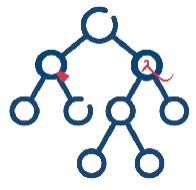
\includegraphics[height=1.0cm]{msca_logo.png}}%
    \end{center}

    \vspace{0.6cm}

    % Main title with Q logos on sides (with clickable links)
    \begin{center}
        \begin{minipage}{0.1\textwidth}
            \centering
            \href{https://quantlet.com}{
\includegraphics[height=1.1cm]{ql_logo.png}}
        \end{minipage}%
        \begin{minipage}{0.78\textwidth}
            \centering
            {\LARGE\bfseries\usebeamercolor[fg]{title}\inserttitle}

            \vspace{0.3cm}

            {\usebeamerfont{subtitle}\usebeamercolor[fg]{title}\insertsubtitle}
        \end{minipage}%
        \begin{minipage}{0.1\textwidth}
            \centering
            \href{https://quantinar.com}{
\includegraphics[height=1.1cm]{qr_logo.png}}
        \end{minipage}
    \end{center}

    \vspace{0.6cm}

    % Authors (left aligned)
    \hspace{0.5cm}{\usebeamerfont{author}\insertauthor}

    \vspace{0.3cm}

    % Institute/Affiliations (left aligned)
    \hspace{0.5cm}\begin{minipage}[t]{0.9\textwidth}
        \raggedright\small\insertinstitute
    \end{minipage}
}

%=============================================================================
% THEOREM ENVIRONMENTS
%=============================================================================
\theoremstyle{definition}
\setbeamertemplate{theorems}[numbered]
\ifdefined\sfmlang
\newtheorem{defn}{Definiție}
\newtheorem{thm}{Teoremă}
\newtheorem{prop}{Propoziție}
\newtheorem{rmk}{Observație}
\else
\newtheorem{defn}{Definition}
\newtheorem{thm}{Theorem}
\newtheorem{prop}{Proposition}
\newtheorem{rmk}{Remark}
\fi

%=============================================================================
% CENTRED MINIPAGE (no extra vertical space)
%=============================================================================
\newenvironment{cminipage}[1]{%
    \par\noindent\hfill\begin{minipage}{#1}\ignorespaces
}{%
    \end{minipage}\hfill\null\par
}

%=============================================================================
% CUSTOM COMMANDS
%=============================================================================
\newcommand{\E}{\mathbb{E}}
\newcommand{\Var}{\text{Var}}
\newcommand{\Cov}{\text{Cov}}
\newcommand{\Corr}{\text{Corr}}
\newcommand{\R}{\mathbb{R}}
\newcommand{\N}{\mathbb{N}}
\newcommand{\Z}{\mathbb{Z}}
\newcommand{\B}{\mathbf{B}}
\newcommand{\imark}{\textcolor{MainBlue}{\textbullet}}
\newcommand{\RMSE}{\text{RMSE}}
\newcommand{\MAE}{\text{MAE}}
\newcommand{\MAPE}{\text{MAPE}}

 se definește
%   \newcommand{\coursename}{Statistics of Financial Markets}      (EN)
%   \newcommand{\coursename}{Statistica piețelor financiare}       (RO)  și  \def\sfmlang{ro}
% Fișierele .tex se află în EN/Courses, EN/Seminars, RO/Cursuri, RO/Seminarii (două niveluri sub rădăcină).
% Deck-urile sînt generate de latex/build_chapterN.py / build_seminarN.py (vezi latex/sfm_build.py).

\documentclass[9pt, aspectratio=169, t]{beamer}
\providecommand{\coursename}{Statistics of Financial Markets}

% Ensure content fits on slides
\setbeamersize{text margin left=8mm, text margin right=8mm}

%=============================================================================
% THEME AND STYLE CONFIGURATION
%=============================================================================
\usetheme{default}
% Using default theme for clean header/footer control

% Color Palette (matching Redispatch PDF)
\definecolor{MainBlue}{RGB}{26, 58, 110}
\definecolor{AccentBlue}{RGB}{26, 58, 110}
\definecolor{IDAred}{RGB}{205, 0, 0}
\definecolor{DarkGray}{RGB}{51, 51, 51}
\definecolor{MediumGray}{RGB}{128, 128, 128}
\definecolor{LightGray}{RGB}{248, 248, 248}
\definecolor{VeryLightGray}{RGB}{235, 235, 235}
\definecolor{KeynoteGray}{RGB}{218, 218, 218}
\definecolor{SectionGray}{RGB}{120, 120, 120}
\definecolor{FooterGray}{RGB}{100, 100, 100}
\definecolor{Crimson}{RGB}{220, 53, 69}
\definecolor{Forest}{RGB}{46, 125, 50}
\definecolor{Amber}{RGB}{181, 133, 63}
\definecolor{Orange}{RGB}{230, 126, 34}
\definecolor{Purple}{RGB}{142, 68, 173}

% Gradient background (exact Keynote 315° gradient: white to RGB 218,218,218)
\setbeamertemplate{background}{%
    \begin{tikzpicture}[remember picture, overlay]
        \shade[shading=axis, shading angle=315,
        top color=white, bottom color=KeynoteGray]
        (current page.south west) rectangle (current page.north east);
    \end{tikzpicture}%
}
% Fallback solid color for compatibility
\setbeamercolor{background canvas}{bg=}

\setbeamercolor{palette primary}{bg=MainBlue, fg=white}
\setbeamercolor{palette secondary}{bg=MainBlue!85, fg=white}
\setbeamercolor{palette tertiary}{bg=MainBlue!70, fg=white}
\setbeamercolor{structure}{fg=MainBlue}
\setbeamercolor{title}{fg=IDAred}
\setbeamercolor{frametitle}{fg=IDAred, bg=}
\setbeamercolor{block title}{bg=MainBlue, fg=white}
\setbeamercolor{block body}{bg=VeryLightGray, fg=DarkGray}
\setbeamercolor{block title alerted}{bg=Crimson, fg=white}
\setbeamercolor{block body alerted}{bg=Crimson!8, fg=DarkGray}
\setbeamercolor{block title example}{bg=Forest, fg=white}
\setbeamercolor{block body example}{bg=Forest!8, fg=DarkGray}
\setbeamercolor{item}{fg=MainBlue}

% Footer colors (override Madrid theme blue)
\setbeamercolor{author in head/foot}{fg=FooterGray, bg=}
\setbeamercolor{title in head/foot}{fg=FooterGray, bg=}
\setbeamercolor{date in head/foot}{fg=FooterGray, bg=}
\setbeamercolor{section in head/foot}{fg=FooterGray, bg=}
\setbeamercolor{subsection in head/foot}{fg=FooterGray, bg=}

% Bullet styles (apply everywhere including blocks)
\setbeamertemplate{itemize item}{\color{MainBlue}$\boxdot$}
\setbeamertemplate{itemize subitem}{\color{MainBlue}$\blacktriangleright$}
\setbeamertemplate{itemize subsubitem}{\color{MainBlue}\tiny$\bullet$}
\setbeamertemplate{itemize/enumerate body begin}{\normalsize}
\setbeamertemplate{itemize/enumerate subbody begin}{\normalsize}

% Item spacing - compact style
\setlength{\leftmargini}{10pt}       % Level 1: minimal indent
\setlength{\leftmarginii}{10pt}      % Level 2: minimal additional indent
% Compact list spacing (zero extra space before/after lists in blocks)
\makeatletter
\def\@listi{\leftmargin\leftmargini \topsep 0pt \parsep 0pt \itemsep 0pt}
\def\@listii{\leftmargin\leftmarginii \topsep 0pt \parsep 0pt \itemsep 0pt}
\makeatother

\setbeamertemplate{navigation symbols}{}

%=============================================================================
% CUSTOM HEADLINE
%=============================================================================
\setbeamertemplate{headline}{%
    \vskip10pt%
    \hbox to \paperwidth{%
        \hskip0.5cm%
        {\small\color{FooterGray}\renewcommand{\hyperlink}[2]{##2}\insertsectionhead}%
        \hfill%
        \textcolor{FooterGray}{\small\insertframenumber}%
        \hskip0.5cm%
    }%
    \vskip4pt%
    {\color{FooterGray}\hrule height 0.4pt}%
}

%=============================================================================
% CUSTOM FOOTER
%=============================================================================
\usepackage{fontawesome5}

\setbeamertemplate{footline}{%
    {\color{FooterGray}\hrule height 0.4pt}%
    \vskip4pt%
    \hbox to \paperwidth{%
        \hskip0.5cm%
        \textcolor{FooterGray}{\small\coursename}%
        \hfill%
        \raisebox{-0.1em}{%
            \begin{tikzpicture}[x=0.08em, y=0.08em, line width=0.4pt]
                \draw[FooterGray] (0,3) -- (1,4) -- (2,3.5) -- (3,5) -- (4,4) -- (5,6) -- (6,5.5) -- (7,4) -- (8,5) -- (9,7) -- (10,6) -- (11,5) -- (12,6.5) -- (13,8) -- (14,7) -- (15,6) -- (16,7.5) -- (17,9) -- (18,8) -- (19,7) -- (20,8.5) -- (21,10) -- (22,9) -- (23,8) -- (24,9.5);
            \end{tikzpicture}%
        }%
        \hskip0.5cm%
    }%
    \vskip6pt%
}

%=============================================================================
% PACKAGES
%=============================================================================
\usepackage[utf8]{inputenc}
\DeclareUnicodeCharacter{03B1}{\ensuremath{\alpha}}
\usepackage[T1]{fontenc}
\usepackage{amsmath, amssymb, amsthm}
\usepackage{mathtools}
\usepackage{bm}
\usepackage{tikz}
\usetikzlibrary{arrows.meta, positioning, shapes, calc, decorations.pathreplacing, shadings}
\usepackage{booktabs}
\usepackage{multirow}
\usepackage{array}
\usepackage{graphicx}
\usepackage{hyperref}
\usepackage{colortbl}
\usepackage{listings}
\lstset{language=Python, basicstyle=\ttfamily\scriptsize, keywordstyle=\color{MainBlue}\bfseries,
  commentstyle=\color{Forest}, stringstyle=\color{Crimson}, breaklines=true,
  frame=none, backgroundcolor=\color{VeryLightGray}, xleftmargin=2mm}
\hypersetup{colorlinks=true, linkcolor=MainBlue, urlcolor=MainBlue}
\graphicspath{{../../logos/}{../../charts/}{../../photos/}}
\usepackage{xcolor}
\hfuzz=2pt  % Suppress tiny overfull warnings (<2pt)
\vfuzz=2pt  % Suppress tiny vertical overfull warnings (<2pt)

%=============================================================================
% QUANTLET COMMANDS
%   \quantlet{<displayed name>}{<url>}       (generic, compatible with the older SFM decks)
%   \sfmquantlet{Ch_05}{SFM_ch5_garch}       -> https://github.com/danpele/SFM/tree/main/Quantlets/Ch_05/SFM_ch5_garch
%   \qlurl{<folder>} is defined per chapter by the generator (Quantlets/Ch_NN/<folder>)
%=============================================================================
\newcommand{\sfmrepo}{https://github.com/danpele/SFM}
\newcommand{\sfmqlbase}{https://github.com/danpele/SFM/tree/main/Quantlets}
\newcommand{\quantlet}[2]{%
    \hfill\href{#2}{%
        \raisebox{-0.15em}{
\includegraphics[height=0.7em]{ql_logo.png}}%
        \textcolor{MainBlue}{\tiny\ #1}%
    }%
}
\newcommand{\sfmquantlet}[2]{\quantlet{\detokenize{#2}}{\sfmqlbase/#1/#2}}

%=============================================================================
% NOTEBOOKS (Google Colab)
%   \colaburl{notebooks/EN/chapter5_seminar_notebook.ipynb} -> the Colab link of a file in the SFM repo
%   \nb: the chapter notebook (each seminar deck redefines it with \renewcommand)
%=============================================================================
\newcommand{\colaburl}[1]{https://colab.research.google.com/github/danpele/SFM/blob/main/#1}
\newcommand{\nb}{https://colab.research.google.com/github/danpele/SFM/tree/main/notebooks/EN}
\newcommand{\nbname}{notebooks/EN}

%=============================================================================
% SLIDE HELPERS (used by the generators; the same as in MFM)
%=============================================================================
% local font size for list bodies (the preamble forces \normalsize)
\newcommand{\itemsize}[1]{\setbeamertemplate{itemize/enumerate body begin}{#1}\setbeamertemplate{itemize/enumerate subbody begin}{#1}}
\newcommand{\intitle}[1]{{\hypersetup{urlcolor=white}#1}}   % white links inside coloured title bars
\newcommand{\imgcap}[1]{{\scriptsize #1}\\[0.5mm]}          % caption under a photo
\newcommand{\imgcredit}[2]{{\tiny\color{FooterGray}\href{#1}{#2}}}   % image credit: source URL, author/licence
\newcommand{\aiprompt}[1]{{\ttfamily\color{MainBlue}#1}}     % a prompt to an AI assistant

%=============================================================================
% SEMINARS: student version by default; the instructor wrapper *_solutions.tex sets \solutionstrue
%=============================================================================
\makeatletter\@ifundefined{ifsolutions}{\expandafter\newif\csname ifsolutions\endcsname}{}\makeatother
\newcommand{\solonly}[1]{\ifsolutions #1\fi}
\newcommand{\propsub}{\ifsolutions\else\framesubtitle{\ifdefined\sfmlang Rezolvarea se discută la seminar\else Solution discussed in class\fi}\fi}

%=============================================================================
% APPENDIX AND CHAPTER LINKS (latex/appendix_links.py writes the calls; it also re-declares these
% macros before \begin{document}, so the decks compile with or without this preamble block)
%=============================================================================
\providecommand{\sfmapplink}[3]{\hypertarget{#2}{}\hyperlink{#1}{\beamergotobutton{#3}}}
\providecommand{\sfmappback}[2]{\begin{tikzpicture}[remember picture,overlay]\node[anchor=south east] at ([xshift=-3mm,yshift=7mm]current page.south east){\hyperlink{#1}{\beamerreturnbutton{#2}}};\end{tikzpicture}}
\providecommand{\sfmchlink}[2]{\href{#1}{#2}}
\providecommand{\sfmchlinkt}[2]{\href{#1}{\usebeamercolor[fg]{frametitle}#2}}

%=============================================================================
% QUANTINAR COMMAND: link către un curs Quantinar (subiecte avansate)
%=============================================================================
\newcommand{\quantinar}[2]{%
    \href{#2}{%
        \raisebox{-0.15em}{
\includegraphics[height=0.8em]{qr_logo.png}}%
        \textcolor{MainBlue}{\scriptsize\ #1}%
    }%
}

%=============================================================================
% CUSTOM TITLE PAGE
%=============================================================================
\defbeamertemplate*{title page}{hybrid}[1][]
{
    \vspace{0.2cm}
    % Logos row - top header (with clickable links)
    \begin{center}
        \href{https://www.ase.ro}{
\includegraphics[height=1.0cm]{ase_logo.png}}\hspace{0.3cm}%
        \href{https://theida.net}{
\includegraphics[height=1.0cm]{ida_logo.png}}\hspace{0.3cm}%
        \href{https://blockchain-research-center.com}{
\includegraphics[height=1.0cm]{brc_logo.png}}\hspace{0.3cm}%
        \href{https://www.ai4efin.ase.ro}{
\includegraphics[height=1.0cm]{ai4efin_logo.png}}\hspace{0.3cm}%
        \href{https://ipe.ro/new}{
\includegraphics[height=1.0cm]{acad_logo.png}}\hspace{0.3cm}%
        \href{https://www.digital-finance-msca.com}{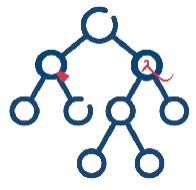
\includegraphics[height=1.0cm]{msca_logo.png}}%
    \end{center}

    \vspace{0.6cm}

    % Main title with Q logos on sides (with clickable links)
    \begin{center}
        \begin{minipage}{0.1\textwidth}
            \centering
            \href{https://quantlet.com}{
\includegraphics[height=1.1cm]{ql_logo.png}}
        \end{minipage}%
        \begin{minipage}{0.78\textwidth}
            \centering
            {\LARGE\bfseries\usebeamercolor[fg]{title}\inserttitle}

            \vspace{0.3cm}

            {\usebeamerfont{subtitle}\usebeamercolor[fg]{title}\insertsubtitle}
        \end{minipage}%
        \begin{minipage}{0.1\textwidth}
            \centering
            \href{https://quantinar.com}{
\includegraphics[height=1.1cm]{qr_logo.png}}
        \end{minipage}
    \end{center}

    \vspace{0.6cm}

    % Authors (left aligned)
    \hspace{0.5cm}{\usebeamerfont{author}\insertauthor}

    \vspace{0.3cm}

    % Institute/Affiliations (left aligned)
    \hspace{0.5cm}\begin{minipage}[t]{0.9\textwidth}
        \raggedright\small\insertinstitute
    \end{minipage}
}

%=============================================================================
% THEOREM ENVIRONMENTS
%=============================================================================
\theoremstyle{definition}
\setbeamertemplate{theorems}[numbered]
\ifdefined\sfmlang
\newtheorem{defn}{Definiție}
\newtheorem{thm}{Teoremă}
\newtheorem{prop}{Propoziție}
\newtheorem{rmk}{Observație}
\else
\newtheorem{defn}{Definition}
\newtheorem{thm}{Theorem}
\newtheorem{prop}{Proposition}
\newtheorem{rmk}{Remark}
\fi

%=============================================================================
% CENTRED MINIPAGE (no extra vertical space)
%=============================================================================
\newenvironment{cminipage}[1]{%
    \par\noindent\hfill\begin{minipage}{#1}\ignorespaces
}{%
    \end{minipage}\hfill\null\par
}

%=============================================================================
% CUSTOM COMMANDS
%=============================================================================
\newcommand{\E}{\mathbb{E}}
\newcommand{\Var}{\text{Var}}
\newcommand{\Cov}{\text{Cov}}
\newcommand{\Corr}{\text{Corr}}
\newcommand{\R}{\mathbb{R}}
\newcommand{\N}{\mathbb{N}}
\newcommand{\Z}{\mathbb{Z}}
\newcommand{\B}{\mathbf{B}}
\newcommand{\imark}{\textcolor{MainBlue}{\textbullet}}
\newcommand{\RMSE}{\text{RMSE}}
\newcommand{\MAE}{\text{MAE}}
\newcommand{\MAPE}{\text{MAPE}}



\newcommand{\qlurl}[1]{https://github.com/danpele/SFM/tree/main/Quantlets/Ch_11/#1}
\renewcommand{\nb}{\colaburl{notebooks/EN/chapter11_seminar_notebook.ipynb}}
\renewcommand{\nbname}{chapter11\_seminar\_notebook.ipynb}
% left column: full width in the student version, narrower next to the solution
\newcommand{\taskw}{\ifsolutions 0.47\textwidth\else 0.96\textwidth\fi}
\newcommand{\solw}{\ifsolutions 0.49\textwidth\else 0pt\fi}

% Clickable citations (DOIs verified via Crossref)

\newcommand{\refPeters}{\href{https://www.wiley.com/en-us/Fractal+Market+Analysis\%3A+Applying+Chaos+Theory+to+Investment+and+Economics-p-9780471585244}{Peters (1994)}}
\newcommand{\refFama}{\href{https://doi.org/10.2307/2325486}{Fama (1970)}}
\newcommand{\refLoAMH}{\href{https://doi.org/10.3905/jpm.2004.442611}{Lo (2004)}}
\newcommand{\refMan}{\href{https://doi.org/10.1086/294632}{Mandelbrot (1963)}}
\newcommand{\refCoast}{\href{https://doi.org/10.1126/science.156.3775.636}{Mandelbrot (1967)}}
\newcommand{\refMVN}{\href{https://doi.org/10.1137/1010093}{Mandelbrot \& Van Ness (1968)}}
\newcommand{\refNoah}{\href{https://doi.org/10.1029/WR004i005p00909}{Mandelbrot \& Wallis (1968)}}
\newcommand{\refMW}{\href{https://doi.org/10.1029/WR005i005p00967}{Mandelbrot \& Wallis (1969)}}
\newcommand{\refHurst}{\href{https://doi.org/10.1061/TACEAT.0006518}{Hurst (1951)}}
\newcommand{\refAL}{\href{https://doi.org/10.1093/biomet/63.1.111}{Anis \& Lloyd (1976)}}
\newcommand{\refLo}{\href{https://doi.org/10.2307/2938368}{Lo (1991)}}
\newcommand{\refNW}{\href{https://doi.org/10.2307/1913610}{Newey \& West (1987)}}
\newcommand{\refTTW}{\href{https://doi.org/10.1016/S0378-3758(98)00250-X}{Teverovsky, Taqqu \& Willinger (1999)}}
\newcommand{\refPeng}{\href{https://doi.org/10.1103/PhysRevE.49.1685}{Peng et al.\ (1994)}}
\newcommand{\refKan}{\href{https://doi.org/10.1016/S0378-4371(01)00144-3}{Kantelhardt et al.\ (2001)}}
\newcommand{\refGPH}{\href{https://doi.org/10.1111/j.1467-9892.1983.tb00371.x}{Geweke \& Porter-Hudak (1983)}}
\newcommand{\refRob}{\href{https://doi.org/10.1214/aos/1176324317}{Robinson (1995)}}
\newcommand{\refGJ}{\href{https://doi.org/10.1111/j.1467-9892.1980.tb00297.x}{Granger \& Joyeux (1980)}}
\newcommand{\refHosking}{\href{https://doi.org/10.1093/biomet/68.1.165}{Hosking (1981)}}
\newcommand{\refBaillie}{\href{https://doi.org/10.1016/0304-4076(95)01732-1}{Baillie (1996)}}
\newcommand{\refDGE}{\href{https://doi.org/10.1016/0927-5398(93)90006-D}{Ding, Granger \& Engle (1993)}}
\newcommand{\refDI}{\href{https://doi.org/10.1016/S0304-4076(01)00073-2}{Diebold \& Inoue (2001)}}
\newcommand{\refGH}{\href{https://doi.org/10.1016/j.jempfin.2003.03.001}{Granger \& Hyung (2004)}}
\newcommand{\refLS}{\href{https://doi.org/10.1080/07350015.1998.10524760}{Lobato \& Savin (1998)}}
\newcommand{\refCobb}{\href{https://doi.org/10.1093/biomet/65.2.243}{Cobb (1978)}}
\newcommand{\refBBM}{\href{https://doi.org/10.1016/S0304-4076(95)01749-6}{Baillie, Bollerslev \& Mikkelsen (1996)}}
\newcommand{\refAB}{\href{https://doi.org/10.1111/j.1540-6261.1997.tb02722.x}{Andersen \& Bollerslev (1997)}}
\newcommand{\refMuller}{\href{https://doi.org/10.1016/S0927-5398(97)00007-8}{Müller et al.\ (1997)}}
\newcommand{\refCorsi}{\href{https://doi.org/10.1093/jjfinec/nbp001}{Corsi (2009)}}
\newcommand{\refWeron}{\href{https://doi.org/10.1016/S0378-4371(02)00961-5}{Weron (2002)}}
\newcommand{\refCT}{\href{https://doi.org/10.1016/j.physa.2003.12.031}{Cajueiro \& Tabak (2004)}}
\newcommand{\refUrq}{\href{https://doi.org/10.1016/j.econlet.2016.09.019}{Urquhart (2016)}}
\newcommand{\refNC}{\href{https://doi.org/10.1016/j.econlet.2016.10.033}{Nadarajah \& Chu (2017)}}
\newcommand{\refBar}{\href{https://doi.org/10.1016/j.econlet.2017.09.013}{Bariviera (2017)}}
\newcommand{\refKrisA}{\href{https://doi.org/10.1142/S0219525912500658}{Kristoufek (2012)}}
\newcommand{\refKrisB}{\href{https://doi.org/10.1038/srep02857}{Kristoufek (2013)}}
\newcommand{\refCarlson}{\href{https://www.federalreserve.gov/pubs/feds/2007/200713/index.html}{Carlson (2007)}}
\newcommand{\refRogers}{\href{https://doi.org/10.1111/1467-9965.00025}{Rogers (1997)}}
\newcommand{\refFHH}{\href{https://doi.org/10.1007/978-3-030-13751-9}{Franke, Härdle \& Hafner (2019)}}
\newcommand{\refWang}{\href{https://doi.org/10.1038/s41586-023-06221-2}{Wang et al.\ (2023)}}
\newcommand{\refPeleA}{\href{https://doi.org/10.1016/j.sbspro.2012.09.1030}{Pele \& Mazurencu-Marinescu (2012)}}
\newcommand{\refPeleB}{\href{https://doi.org/10.5018/economics-ejournal.ja.2019-29}{Pele \& Mazurencu-Marinescu-Pele (2019)}}

\title[Statistica piețelor financiare]{Statistica piețelor financiare}
\subtitle{Seminarul 11: Ipoteza piețelor fractale și memoria lungă\ifsolutions\ (versiunea profesorului)\fi}
\author[D.T. Pele]{Daniel Traian PELE}
\institute{Academia de Studii Economice din București\\
IDA Institute Digital Assets\\
Blockchain Research Center\\
AI4EFin Artificial Intelligence for Energy Finance\\
Academia Română, Institutul de Prognoză Economică\\
MSCA Digital Finance}
\date{}

%=============================================================================
\providecommand{\sfmapplink}[3]{\hypertarget{#2}{}\hyperlink{#1}{\beamergotobutton{#3}}}  % APPLINKS-MACROS
\providecommand{\sfmappback}[2]{\begin{tikzpicture}[remember picture,overlay]\node[anchor=south east] at ([xshift=-3mm,yshift=7mm]current page.south east){\hyperlink{#1}{\beamerreturnbutton{#2}}};\end{tikzpicture}}  % APPLINKS-MACROS
\providecommand{\sfmchlink}[2]{\href{#1}{#2}}  % APPLINKS-MACROS
\providecommand{\sfmchlinkt}[2]{\href{#1}{\usebeamercolor[fg]{frametitle}#2}}  % APPLINKS-MACROS
\begin{document}
%=============================================================================

{
\setbeamertemplate{headline}{}
\setbeamertemplate{footline}{}
\begin{frame}[noframenumbering]
    \titlepage
\end{frame}
}
% BEGIN-ACRONYMS (generat de latex/acronyms.py; nu editati manual)
\begin{frame}{Acronime folosite în acest material}
\setbeamertemplate{itemize/enumerate body begin}{\tiny}
\begin{columns}[T]
\begin{column}{0.49\textwidth}
\begin{itemize}\setlength{\itemsep}{0pt}
    \item \textbf{ACF}: Autocorrelation Function (funcția de autocorelație)
    \item \textbf{AI}: Artificial Intelligence (inteligență artificială)
    \item \textbf{AR}: AutoRegressive (model); in event studies: Abnormal Return (model autoregresiv; în studiile de eveniment: randament anormal)
    \item \textbf{ARFIMA}: AutoRegressive Fractionally Integrated Moving Average (model autoregresiv fracționar integrat cu medie mobilă)
    \item \textbf{BET}: Bucharest Exchange Trading (index) — indicele de referință al Bursei de Valori București
    \item \textbf{BVB}: Bursa de Valori București
    \item \textbf{DFA}: Detrended Fluctuation Analysis (analiza fluctuațiilor fără tendință)
    \item \textbf{EMH}: Efficient Market Hypothesis (ipoteza pieței eficiente)
    \item \textbf{EODHD}: EOD Historical Data (market-data provider) — furnizor de date de piață
    \item \textbf{FMH}: Fractal Market Hypothesis (ipoteza pieței fractale)
    \item \textbf{GARCH}: Generalised AutoRegressive Conditional Heteroskedasticity (heteroscedasticitate condiționată autoregresivă generalizată)
    \item \textbf{GPH}: Geweke–Porter-Hudak (log-periodogram estimator) — estimatorul Geweke–Porter-Hudak pe log-periodogramă
    \item \textbf{MA}: Moving Average (medie mobilă)
\end{itemize}
\end{column}
\begin{column}{0.49\textwidth}
\begin{itemize}\setlength{\itemsep}{0pt}
    \item \textbf{OLS}: Ordinary Least Squares (metoda celor mai mici pătrate)
    \item \textbf{SE}: Standard Error (eroare standard)
\end{itemize}
\end{column}
\end{columns}
\end{frame}
% END-ACRONYMS

\begin{frame}{Întrebarea de azi și traseul}
\itemsize{\small}
\begin{itemize}
    \item \textbf{Întrebarea}: cum putem măsura memoria lungă a unei piețe fără să vedem memorie acolo unde nu există?
    \begin{itemize}
        \item seminarul are loc \textbf{înaintea} Cursului 11: secțiunea „Noțiuni necesare azi” dă toate definițiile folosite în cerințe
    \end{itemize}
    \item Traseul
    \begin{itemize}
        \item Partea A: R/S pas cu pas, exponentul Hurst dintr-un grafic R/S, zgomotul gaussian fracționar și scalarea riscului, ponderile și autocorelațiile ARFIMA, pe hîrtie
        \item Partea B: R/S, DFA, GPH și testul lui Lo cu benzi Monte Carlo pe S\&P 500, BET, Banca Transilvania și Bitcoin; memoria lungă a volatilității; exponenți pe ferestre mobile; fiecare cu o întrebare de interpretare
        \item Partea C: o întrebare deschisă pentru proiect și un răspuns AI de verificat
    \end{itemize}
    \item Notebook-ul de azi: \href{\nb}{deschideți notebook-ul seminarului în Google Colab}; fiecare cerință indică secțiunea din notebook
    \item Seminarul are rol de exercițiu și nu se notează; rezolvările cerințelor [Propus] se discută la seminar
\end{itemize}
\end{frame}

\begin{frame}{Harta exercițiilor}
\itemsize{\small}
\begin{center}
\footnotesize
\begin{tabular}{>{\raggedright\arraybackslash}p{1.1cm}>{\raggedright\arraybackslash}p{7.5cm}>{\raggedright\arraybackslash}p{1.9cm}>{\raggedright\arraybackslash}p{1.4cm}}
\toprule
\textbf{Cerința} & \textbf{Întrebarea} & \textbf{Tipul} & \textbf{Model} \\
\midrule
A1, A2 & R/S pentru opt randamente, pas cu pas; $H$ din trei puncte ale unui grafic R/S & Rezolvat, Propus & A1 \\
A3, A4 & zgomot gaussian fracționar: autocorelații, riscul pe 10 zile, VaR 1\% (value at risk, valoarea expusă la risc) & Rezolvat, Propus & A3 \\
A5, A6 & ARFIMA(0,$d$,0): ponderi și autocorelații comparate cu un AR(1) & Rezolvat, Propus & A5 \\
B1, B2 & R/S, DFA, GPH și testul lui Lo cu benzi Monte Carlo: S\&P 500; BET, TLV & Rezolvat, Propus & B1 \\
B3, B4 & memoria lungă a lui $|r_t|$ și $r_t^2$, testul permutării: S\&P 500; Bitcoin & Rezolvat, Propus & B3 \\
B5, B6 & exponenți DFA pe ferestre mobile, cu o bandă Monte Carlo: S\&P 500; DAX, TLV & Rezolvat, Propus & B5 \\
C1, C2 & se schimbă memoria în crize? ce este greșit într-un răspuns AI? & Propus & B1, B3 \\
\bottomrule
\end{tabular}
\end{center}
\begin{itemize}
    \item \textbf{[Rezolvat]}: rezolvarea completă în slide-uri și în notebook, un model de urmat; \textbf{[Propus]}: îl rezolvați voi, după model
\end{itemize}
\end{frame}

\begin{frame}{Datele folosite}
\itemsize{\small}
\begin{center}
\footnotesize
\begin{tabular}{llll}
\toprule
\textbf{Seria} & \textbf{Sursa} & \textbf{Prețul folosit} & \textbf{Perioada} \\
\midrule
S\&P 500, DAX, BET & EODHD & închidere & 2000--2026 \\
Bitcoin & EODHD & închidere, 7 zile pe săptămînă & 2014--2026 \\
Banca Transilvania (TLV) & EODHD & închidere ajustată & 2010--2026 \\
\bottomrule
\end{tabular}
\end{center}
\begin{itemize}
    \item Randamente logaritmice zilnice în \%: $r_t = 100\,(\ln P_t - \ln P_{t-1})$; weekendurile și închiderile repetate din zilele libere se elimină (cu excepția Bitcoin); ultima zi este 18 septembrie 2026
    \item TLV: zilele de 30 și 31 mai 2016 se elimină (o ajustare de preț aplicată cu o zi mai tîrziu, \sfmchlink{https://danpele.github.io/SFM/RO/Cursuri/capitol2_distributii_clasice_fapte_stilizate.pdf}{Capitolul 2})
    \item În notebook: \texttt{returns('bet')}, \texttt{hurst\_rs(x)}, \texttt{hurst\_dfa(x)}, \texttt{gph(x)}, \texttt{lo\_test(x)}, \texttt{mc\_null(N)}; nu este nevoie de cont sau de cheie
\end{itemize}
\end{frame}


%=============================================================================
\section{Noțiuni necesare azi}
%=============================================================================

\begin{frame}{Noțiuni necesare azi (1/5): ipoteza pieței fractale și $H$}
\itemsize{\small}
\begin{itemize}
    \item \textbf{FMH} (fractal market hypothesis, ipoteza pieței fractale) \refPeters: o piață este stabilă cînd investitori cu multe orizonturi (de la minute la decenii) tranzacționează între ei
    \begin{itemize}
        \item într-o criză, toate orizonturile se reduc la cel mai scurt: fără cumpărători, fără lichiditate
        \item testabilă prin scalare și memorie pe orizonturi diferite
    \end{itemize}
    \item \textbf{Autosimilaritate}: $X_{ct} \overset{d}{=} c^H X_t$; abaterea standard pe $h$ zile este de $h^H$ ori cea zilnică
    \begin{itemize}
        \item \textbf{Exponentul Hurst} $H \in (0, 1)$: $H = 0{,}5$ creșteri independente (mers aleator, EMH); $H > 0{,}5$ persistență; $H < 0{,}5$ antipersistență
        \item $H$ nu este o probabilitate; dimensiunea fractală a unei traiectorii de preț este $D = 2 - H$
    \end{itemize}
\end{itemize}
\end{frame}

\begin{frame}{Noțiuni necesare azi (2/5): statistica R/S}
\itemsize{\small}
\begin{itemize}
    \item Blocul $x_1, \dots, x_n$, media $\bar x$; abaterile cumulate $Y_k = \sum_{j=1}^{k}(x_j - \bar x)$
    \begin{itemize}
        \item amplitudinea $R_n = \max_k Y_k - \min_k Y_k$; abaterea standard $S_n = \sqrt{\tfrac1n\sum_j(x_j - \bar x)^2}$; $(R/S)_n = R_n/S_n$ \refHurst
    \end{itemize}
    \item $(R/S)_n \approx c\,n^H$: facem media $R/S$ pe blocuri fără suprapunere de mărime $n$, apoi estimăm regresia lui $\log(R/S)_n$ pe $\log n$; panta este $\hat H$
    \begin{itemize}
        \item trei mărimi de bloc la distanțe egale pe scară logaritmică: panta OLS este egală cu panta dintre punctele extreme
    \end{itemize}
    \item Eșantioane mici: pentru date i.i.d., panta R/S este peste 0,5 (circa $0{,}544$ pentru $N = 6\,714$) \refAL
\end{itemize}
\end{frame}

\begin{frame}{Noțiuni necesare azi (3/5): memoria lungă, fGn și ARFIMA}
\itemsize{\footnotesize}
\begin{itemize}
    \item \textbf{Memoria lungă}: $\rho(k) \sim C\,k^{2d - 1}$, $0 < d < 0{,}5$; autocorelațiile scad hiperbolic și nu sînt sumabile (\refFHH, 14.1); memoria scurtă (AR): $\rho(k) = \phi^k$
    \item \textbf{Zgomotul gaussian fracționar} (fGn, fractional Gaussian noise), creșterile mișcării browniene fracționare \refMVN:
    \begin{itemize}
        \item $\rho(k) = \tfrac12\left(|k + 1|^{2H} - 2|k|^{2H} + |k - 1|^{2H}\right) \approx H(2H - 1)k^{2H - 2}$; $\rho(1) = 2^{2H - 1} - 1$
    \end{itemize}
    \item \textbf{ARFIMA}(0,$d$,0) \refHosking: $(1 - L)^d X_t = \varepsilon_t$, $d = H - 0{,}5$
    \begin{itemize}
        \item $(1 - L)^d = \sum_j \pi_j L^j$: $\pi_0 = 1$, $\pi_j = \pi_{j-1}(j - 1 - d)/j$; ponderile MA $\psi_j = \psi_{j-1}(j - 1 + d)/j$
        \item $\rho(1) = d/(1 - d)$, $\rho(k) = \rho(k - 1)\,(k - 1 + d)/(k - d)$
    \end{itemize}
\end{itemize}
\end{frame}

\begin{frame}{Noțiuni necesare azi (4/5): DFA, GPH, testul lui Lo și benzile Monte Carlo}
\itemsize{\footnotesize}
\begin{itemize}
    \item \textbf{DFA} \refPeng: profilul $Y_k$; o dreaptă estimată în fiecare bloc de mărime $n$; $F(n)$ = rădăcina mediei pătratelor abaterilor; panta lui $\log F$ în funcție de $\log n$ = $\hat H$
    \item \textbf{GPH} \refGPH: OLS pentru $\ln I(\lambda_j)$ (periodograma) în funcție de $-\ln(4\sin^2(\lambda_j/2))$, $j \le m = \lfloor T^{0{,}5}\rfloor$; panta $\hat d$, SE $\pi/\sqrt{24m}$
    \item \textbf{R/S modificat al lui Lo} \refLo: $V = R/(\sqrt{N}\hat\sigma(q))$, cu o varianță Newey--West; $H_0$: memorie scurtă; respingem la 5\% dacă $V \notin [0{,}809, 1{,}862]$
    \item \textbf{Banda Monte Carlo} \refWeron: simulăm multe serii i.i.d.\ Normale de aceeași lungime, aplicăm același estimator, luăm cuantilele de 2,5\% și 97,5\%
    \begin{itemize}
        \item respingem $H = 0{,}5$ doar dacă $\hat H$ se află în afara benzii
    \end{itemize}
\end{itemize}
\end{frame}

\begin{frame}{Noțiuni necesare azi (5/5): memorie aparentă, volatilitate, ferestre mobile}
\itemsize{\small}
\begin{itemize}
    \item \textbf{Memorie lungă aparentă}: schimbările mediei \refDI\ și volatilitatea GARCH persistentă (\sfmchlink{https://danpele.github.io/SFM/RO/Cursuri/capitol9_modele_arch_garch.pdf}{Capitolul 9}) produc ACF de selecție care scad lent
    \item \textbf{Testul permutării}: o permutare aleatoare păstrează distribuția și distruge ordinea; dacă $\hat H$ scade la 0,5, memoria era în ordinea zilelor
    \item \textbf{Volatilitatea}: memoria lungă a lui $|r_t|$ și $r_t^2$ \refDGE\ privește mărimea randamentelor, nu direcția lor
    \item \textbf{Ferestre mobile}: $\hat H$ pe ferestre de 1000 de zile mutate cu 21, datat la sfîrșitul ferestrei; cu teste la 5\%, circa 5\% dintre ferestre ies din bandă din întîmplare
\end{itemize}
\end{frame}


%=============================================================================
\section{Partea A: calcule pe hîrtie}
%=============================================================================

\begin{frame}{A1: R/S pas cu pas [Rezolvat]}
\itemsize{\scriptsize}
\begin{columns}[T]
\begin{column}{0.47\textwidth}
\begin{block}{Cerință}
\begin{itemize}
    \item Opt randamente zilnice (\%): $0{,}5;\ -0{,}3;\ 0{,}8;\ -0{,}2;\ 0{,}6;\ -0{,}1;\ 0{,}4;\ -0{,}7$.
    \item 1. Calculați media, abaterile și abaterile cumulate $Y_1, \dots, Y_8$.
    \item 2. Calculați $R$, $S$ (cu numitorul $n$) și $R/S$.
    \item 3. Randamentele S\&P 500 din 2000 dau $(R/S)_{16} = 3{,}91$, $(R/S)_{64} = 8{,}38$, $(R/S)_{256} = 17{,}03$; calculați $\hat H$.
    \item Raportați: $R$, $S$, $R/S$, $\hat H$ și o frază.
\end{itemize}
\end{block}
\end{column}
\begin{column}{0.49\textwidth}
\begin{exampleblock}{Rezolvare}
\begin{itemize}
    \item 1. $\bar x = 0{,}125$; $Y_k$: $0{,}375$; $-0{,}050$; $0{,}625$; $0{,}300$; $0{,}775$; $0{,}550$; $0{,}825$; $0{,}000$
    \item 2. $R = 0{,}825 - (-0{,}050) = 0{,}875$; $S = \sqrt{1{,}915/8} = 0{,}489$; $R/S = 1{,}788$
    \item 3. $\log_{10}$: $n$: $1{,}204$; $1{,}806$; $2{,}408$; $R/S$: $0{,}592$; $0{,}923$; $1{,}231$; $\hat H = 0{,}639/1{,}204 = 0{,}531$
    \item Semnele alternante țin abaterile cumulate mici; un $\hat H$ puțin peste 0,5 reflectă deplasarea R/S în eșantioane mici, nu memoria (B1).
\end{itemize}
\end{exampleblock}
\end{column}
\end{columns}
\end{frame}

\begin{frame}{A2: semne grupate [Propus]}
\propsub
\itemsize{\scriptsize}
\begin{columns}[T]
\begin{column}{\taskw}
\begin{block}{Cerință}
\begin{itemize}
    \item Opt randamente (\%): $0{,}6;\ 0{,}4;\ 0{,}5;\ 0{,}3;\ -0{,}4;\ -0{,}6;\ -0{,}2;\ -0{,}5$. Model: A1.
    \item 1. Calculați media și $Y_1, \dots, Y_8$.
    \item 2. Calculați $R$, $S$ și $R/S$ și comparați cu A1.
    \item 3. Randamentele BET dau $(R/S)_{16} = 4{,}23$, $(R/S)_{64} = 10{,}08$, $(R/S)_{256} = 21{,}61$; calculați $\hat H$.
    \item Raportați: $R/S$, $\hat H$ și două fraze.
\end{itemize}
\end{block}
\end{column}
\begin{column}{\solw}
\solonly{%
\begin{exampleblock}{Rezolvare}
\begin{itemize}
    \item 1. $\bar x = 0{,}0125$; $Y_k$: $0{,}5875$; $0{,}9750$; $1{,}4625$; $1{,}7500$; $1{,}3375$; $0{,}7250$; $0{,}5125$; $0{,}0000$
    \item 2. $R = 1{,}750$, $S = 0{,}457$, $R/S = 3{,}832$, aproape dublu față de A1 ($1{,}788$)
    \item 3. $\hat H = (1{,}335 - 0{,}626)/1{,}204 = 0{,}588$
    \item Seriile de semne egale fac ca abaterile cumulate să se îndepărteze de zero: un $R/S$ mare este semnul persistenței; BET este peste S\&P 500 (A1).
\end{itemize}
\end{exampleblock}
}
\end{column}
\end{columns}
\end{frame}

\begin{frame}{A3: zgomot gaussian fracționar și riscul pe 10 zile [Rezolvat]}
\itemsize{\scriptsize}
\begin{columns}[T]
\begin{column}{0.47\textwidth}
\begin{block}{Cerință}
\begin{itemize}
    \item Randamentele zilnice urmează un fGn cu $H = 0{,}7$ și volatilitatea zilnică $\sigma = 1{,}2\%$; $z_{0{,}99} = 2{,}326$.
    \item 1. Calculați exact $\rho(1)$ și $\rho(10)$, precum și $\rho(10)$ cu aproximarea $H(2H - 1)k^{2H - 2}$.
    \item 2. Calculați factorul de scalare $10^H$ și comparați-l cu $\sqrt{10}$.
    \item 3. Calculați VaR 1\% pe o zi și pe 10 zile (cazul Normal), cu $h^H$ și cu $\sqrt{h}$.
    \item 4. Calculați dimensiunea fractală a traiectoriei prețului.
    \item Raportați: șase valori și o frază.
\end{itemize}
\end{block}
\end{column}
\begin{column}{0.49\textwidth}
\begin{exampleblock}{Rezolvare}
\begin{itemize}
    \item 1. $\rho(1) = 2^{0{,}4} - 1 = 0{,}320$; $\rho(10) = \tfrac12(11^{1{,}4} - 2 \cdot 10^{1{,}4} + 9^{1{,}4}) = 0{,}0704$; aproximarea $0{,}7 \cdot 0{,}4 \cdot 10^{-0{,}6} = 0{,}0703$
    \item 2. $10^{0{,}7} = 5{,}012$, față de $\sqrt{10} = 3{,}162$
    \item 3. $2{,}326 \times 1{,}2 = 2{,}79\%$; 10 zile: $2{,}79 \times 5{,}012 = 13{,}99\%$, față de $8{,}83\%$ ($+58{,}5\%$)
    \item 4. $D = 2 - H = 1{,}30$
    \item Randamentele persistente fac ca pierderile pe mai multe zile să se adune: regula $\sqrt{h}$ subestimează riscul pe 10 zile cu peste o treime.
\end{itemize}
\end{exampleblock}
\end{column}
\end{columns}
\end{frame}

\begin{frame}{A4: antipersistență și o abatere mică de la 0,5 [Propus]}
\propsub
\itemsize{\scriptsize}
\begin{columns}[T]
\begin{column}{\taskw}
\begin{block}{Cerință}
\begin{itemize}
    \item Datele din A3, cu $H = 0{,}4$ și cu $H = 0{,}55$. Model: A3.
    \item 1. Calculați $\rho(1)$ și $\rho(10)$ pentru ambele valori ale lui $H$.
    \item 2. Calculați VaR 1\% pe 10 zile pentru ambele valori și diferența față de regula $\sqrt{h}$, în \%.
    \item 3. Calculați $D$ pentru ambele valori.
    \item Raportați: opt valori și o frază.
\end{itemize}
\end{block}
\end{column}
\begin{column}{\solw}
\solonly{%
\begin{exampleblock}{Rezolvare}
\begin{itemize}
    \item 1. $H = 0{,}4$: $\rho(1) = -0{,}129$, $\rho(10) = -0{,}0051$; $H = 0{,}55$: $0{,}072$, $0{,}0069$
    \item 2. $H = 0{,}4$: $7{,}01\%$ ($-20{,}6\%$); $H = 0{,}55$: $9{,}90\%$ ($+12{,}2\%$); regula $\sqrt{h}$: $8{,}83\%$
    \item 3. $D = 1{,}60$ și $1{,}45$
    \item O autocorelație zilnică de doar $0{,}072$ schimbă deja riscul pe 10 zile cu $12{,}2\%$.
\end{itemize}
\end{exampleblock}
}
\end{column}
\end{columns}
\end{frame}

\begin{frame}{A5: ARFIMA(0; 0,3; 0) comparat cu un AR(1) [Rezolvat]}
\itemsize{\scriptsize}
\begin{columns}[T]
\begin{column}{0.47\textwidth}
\begin{block}{Cerință}
\begin{itemize}
    \item $(1 - L)^{0{,}3}X_t = \varepsilon_t$, $\varepsilon_t$ i.i.d.\ $N(0, 1)$.
    \item 1. Calculați $\pi_1$, $\pi_2$ și ponderile MA $\psi_1$, $\psi_2$.
    \item 2. Calculați $\rho(1)$, $\rho(2)$, $\rho(10)$ și $\rho(50)$.
    \item 3. Pentru un AR(1) cu $\phi = \rho(1)$, calculați $\rho(10)$ și $\rho(50)$.
    \item 4. Dați $H$ și primul decalaj cu $\rho(k) < 0{,}05$ pentru ambele modele.
    \item Raportați: zece valori și o frază.
\end{itemize}
\end{block}
\end{column}
\begin{column}{0.49\textwidth}
\begin{exampleblock}{Rezolvare}
\begin{itemize}
    \item 1. $\pi_1 = -0{,}3$, $\pi_2 = -0{,}3 \times 0{,}7/2 = -0{,}105$; $\psi_1 = 0{,}3$, $\psi_2 = 0{,}3 \times 1{,}3/2 = 0{,}195$
    \item 2. $\rho(1) = 0{,}3/0{,}7 = 0{,}429$; $\rho(2) = 0{,}429 \times 1{,}3/1{,}7 = 0{,}328$; $\rho(10) = 0{,}173$; $\rho(50) = 0{,}091$
    \item 3. $0{,}429^{10} = 0{,}0002$; $0{,}429^{50} \approx 0$
    \item 4. $H = 0{,}8$; sub 0,05 după 4 decalaje (AR) și 222 de decalaje (ARFIMA)
    \item Același $\rho(1)$, memorie foarte diferită: AR(1) uită în cîteva zile, ARFIMA în cîteva luni.
\end{itemize}
\end{exampleblock}
\end{column}
\end{columns}
\end{frame}

\begin{frame}{A6: memorie puternică și antipersistență [Propus]}
\propsub
\itemsize{\scriptsize}
\begin{columns}[T]
\begin{column}{\taskw}
\begin{block}{Cerință}
\begin{itemize}
    \item ARFIMA(0,$d$,0) cu $d = 0{,}45$ și cu $d = -0{,}2$. Model: A5.
    \item 1. Calculați $\pi_1$, $\pi_2$, $\rho(1)$, $\rho(2)$ și $\rho(10)$ pentru ambele valori.
    \item 2. Pentru $d = 0{,}45$, comparați $\rho(10)$ și $\rho(50)$ cu un AR(1) cu $\phi = \rho(1)$.
    \item 3. Dați $H$ pentru ambele valori și precizați care este staționar.
    \item Raportați: un tabel mic și o frază.
\end{itemize}
\end{block}
\end{column}
\begin{column}{\solw}
\solonly{%
\begin{exampleblock}{Rezolvare}
\begin{itemize}
    \item 1. $d = 0{,}45$: $\pi_1 = -0{,}450$, $\pi_2 = -0{,}124$, $\rho(1) = 0{,}818$, $\rho(2) = 0{,}765$, $\rho(10) = 0{,}652$
    \item $d = -0{,}2$: $\pi_1 = 0{,}200$, $\pi_2 = 0{,}120$, $\rho(1) = -0{,}167$, $\rho(2) = -0{,}061$, $\rho(10) = -0{,}006$
    \item 2. ARFIMA: $\rho(10) = 0{,}652$, $\rho(50) = 0{,}555$; AR(1): $0{,}1344$, $0{,}00004$; sub 0,05 după 15 decalaje (AR); încă peste 0,05 la decalajul 2000 (ARFIMA)
    \item 3. $H = 0{,}95$ și $H = 0{,}3$; ambele staționare ($|d| < 0{,}5$); $d = -0{,}2$ este antipersistent.
\end{itemize}
\end{exampleblock}
}
\end{column}
\end{columns}
\end{frame}


%=============================================================================
\section{Partea B: date reale, inferență și interpretare}
%=============================================================================

\begin{frame}{B1: memorie lungă în randamentele S\&P 500? [Rezolvat]}
\itemsize{\footnotesize}
\begin{itemize}
\item \textbf{Întrebarea}: au randamentele zilnice S\&P 500 memorie lungă?
\item \textbf{Date}: închiderile S\&P 500 din 2000, randamente logaritmice zilnice în \%
\item \textbf{Cerințe}
\begin{enumerate}
    \item Estimați $H$ cu R/S și DFA (mărimi de bloc de la 10 la $N/4$) și $d$ cu GPH ($m = \lfloor T^{0{,}5}\rfloor$), cu eroarea standard a lui $\hat d$.
    \item Calculați statistica modificată a lui Lo, $V(q)$, cu $q$ ales prin regula lui Andrews, și statistica clasică $V(0)$.
    \item Simulați 300 de serii i.i.d.\ Normale de aceeași lungime și dați banda de 95\% a fiecărui estimator.
    \item Desenați graficul R/S în interiorul anvelopei Monte Carlo.
    \item Interpretare: este estimarea R/S de peste 0,5 o dovadă de memorie lungă?
\end{enumerate}
\item \textbf{Raportați}: un tabel cu patru estimări și benzile lor, graficul și două fraze
\item Notebook: secțiunea B1
\end{itemize}
\end{frame}

\begin{frame}{B1: rezolvare [Rezolvat]}
\itemsize{\scriptsize}
\begin{center}
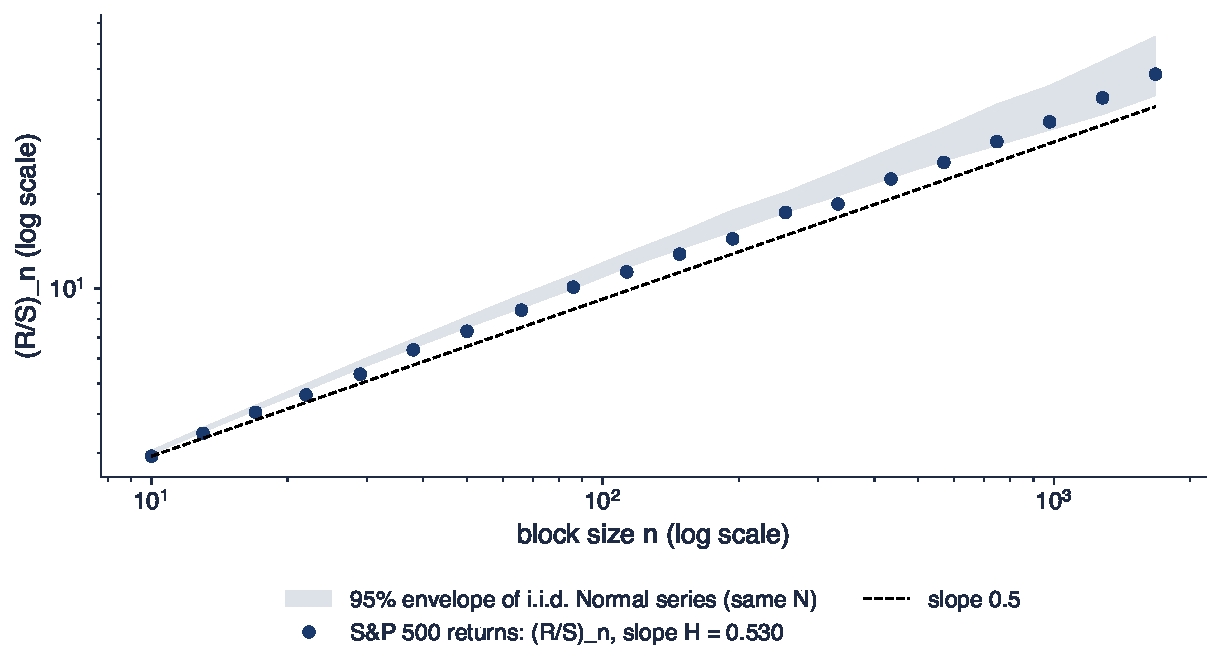
\includegraphics[width=0.96\textwidth,height=0.30\textheight,keepaspectratio]{ch11_sem_b1.pdf}
\end{center}
\vspace{-2mm}
\begin{center}
\scriptsize
\begin{tabular}{lrrrr}
\toprule
 & R/S & DFA & GPH $\hat H = \hat d + 0{,}5$ & Lo $V(q)$ \\
\midrule
estimare & $0{,}530$ & $0{,}488$ & $0{,}536$ & $1{,}559$ ($q = 7$) \\
banda de 95\% & $[0{,}512; 0{,}575]$ & $[0{,}456; 0{,}540]$ & $[0{,}363; 0{,}652]$ & $[0{,}809, 1{,}862]$ \\
\bottomrule
\end{tabular}
\end{center}
\begin{itemize}
    \item $N = 6\,714$; GPH: $\hat d = 0{,}036$, SE $0{,}071$ ($m = 81$), $t = 0{,}51$; statistica clasică $V(0) = 1{,}379$
    \item Interpretare: nu: seriile i.i.d.\ de această lungime dau în medie R/S $0{,}544$; fiecare estimare se află în banda ei, iar testul lui Lo nu respinge memoria scurtă
\end{itemize}\sfmquantlet{Ch_11}{SFM_ch11_seminar}
\end{frame}

\begin{frame}{B2: BET și Banca Transilvania [Propus]}
\itemsize{\footnotesize}
\begin{itemize}
\item \textbf{Întrebarea}: arată BET sau Banca Transilvania memorie lungă în randamente? Model: B1.
\item \textbf{Date}: BET din 2000, TLV din 2010 (fără 30--31 mai 2016); randamente logaritmice zilnice în \%
\item \textbf{Cerințe}
\begin{enumerate}
    \item Estimați $H$ cu R/S, DFA și GPH pentru fiecare serie.
    \item Calculați $V(q)$ al lui Lo și precizați dacă memoria scurtă este respinsă la 5\%.
    \item Calculați banda Monte Carlo a fiecărui estimator pentru fiecare lungime.
    \item Interpretare: ce ar putea explica rezultatul pentru BET?
\end{enumerate}
\item \textbf{Raportați}: un tabel și două fraze
\item Notebook: secțiunea B2
\end{itemize}
\end{frame}

\ifsolutions
\begin{frame}{B2: rezolvare [Propus]}
\itemsize{\footnotesize}
\begin{center}
\scriptsize
\begin{tabular}{lrrrrr}
\toprule
 & $N$ & R/S [banda] & DFA [banda] & GPH $\hat d$ (SE) & Lo $V(q)$ \\
\midrule
BET & 6\,670 & $0{,}578$ $[0{,}507; 0{,}578]$ & $0{,}570$ $[0{,}451; 0{,}542]$ & $0{,}166$ ($0{,}071$) & $1{,}961$ \\
TLV & 3\,788 & $0{,}539$ $[0{,}509; 0{,}590]$ & $0{,}473$ $[0{,}442; 0{,}551]$ & $-0{,}063$ ($0{,}082$) & $1{,}071$ \\
\bottomrule
\end{tabular}
\end{center}
\begin{itemize}
    \item BET: R/S la limita benzii, DFA peste ea, $\hat d$ GPH la circa 2{,}33 erori standard de 0, testul lui Lo respinge ($1{,}961 > 1{,}862$): persistență
    \item TLV: fiecare estimare se află în banda ei; testul lui Lo nu respinge
    \item Interpretare: tranzacționarea redusă și ajustarea lentă a prețurilor în primii ani ai BVB (\sfmchlink{https://danpele.github.io/SFM/RO/Cursuri/capitol7_piete_eficiente_mers_aleator_vr.pdf}{Capitolul 7}, testele raportului varianțelor); exponenții pe ferestre mobile din curs arată că BET se apropie de 0,5
\end{itemize}\sfmquantlet{Ch_11}{SFM_ch11_seminar}
\end{frame}
\fi

\begin{frame}{B3: memoria lungă a volatilității S\&P 500 [Rezolvat]}
\itemsize{\footnotesize}
\begin{itemize}
\item \textbf{Întrebarea}: au randamentele absolute și pătratele randamentelor S\&P 500 memorie lungă?
\item \textbf{Date}: randamentele logaritmice zilnice S\&P 500 din 2000; $|r_t|$ și $r_t^2$
\item \textbf{Cerințe}
\begin{enumerate}
    \item Estimați $d$ cu GPH pentru $m = \lfloor T^{0{,}5}\rfloor$ și $m = \lfloor T^{0{,}6}\rfloor$ și $H$ cu DFA, pentru $|r_t|$ și $r_t^2$.
    \item Raportați ACF a lui $|r_t|$ la decalajele 1, 50 și 250 și banda de 95\% $\pm 1{,}96/\sqrt{T}$.
    \item Permutați aleator $|r_t|$ și repetați estimările.
    \item Desenați ACF a lui $|r_t|$ înainte și după permutare.
    \item Interpretare: contrazice memoria lungă a lui $|r_t|$ forma slabă a EMH?
\end{enumerate}
\item \textbf{Raportați}: un tabel, graficul și două fraze
\item Notebook: secțiunea B3
\end{itemize}
\end{frame}

\begin{frame}{B3: rezolvare [Rezolvat]}
\itemsize{\scriptsize}
\begin{center}
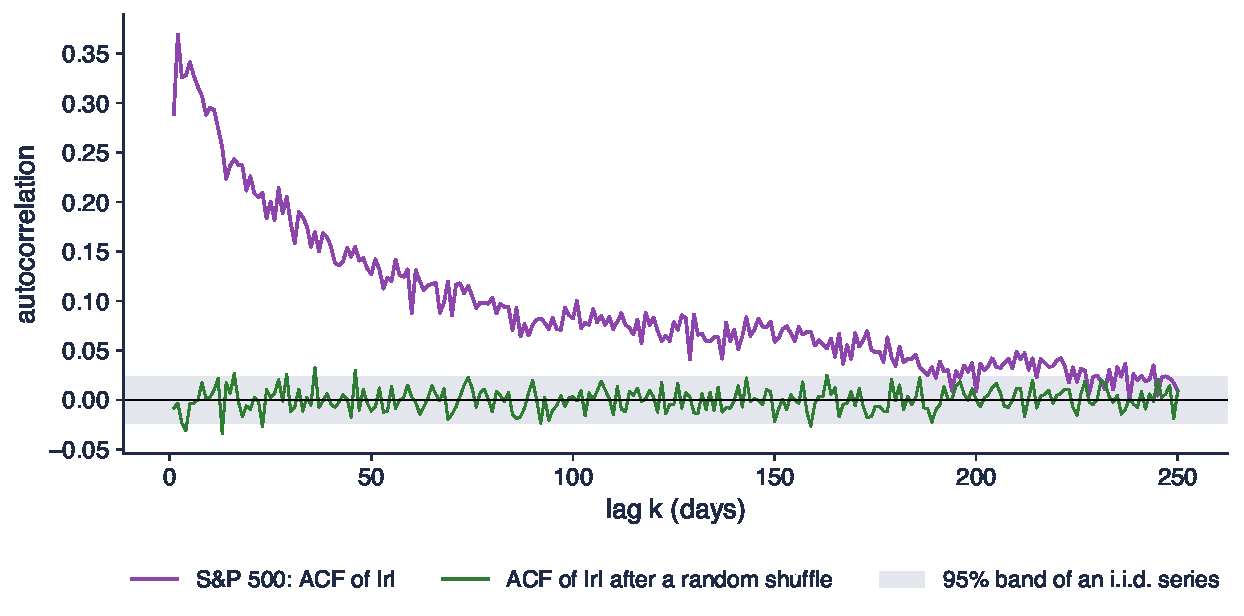
\includegraphics[width=0.96\textwidth,height=0.28\textheight,keepaspectratio]{ch11_sem_b3.pdf}
\end{center}
\vspace{-2mm}
\begin{center}
\scriptsize
\begin{tabular}{lrrrrrr}
\toprule
 & GPH $T^{0{,}5}$ & GPH $T^{0{,}6}$ & DFA & $\rho(1)$ & $\rho(50)$ & $\rho(250)$ \\
\midrule
$|r_t|$ & $0{,}470$ & $0{,}467$ & $0{,}953$ & $0{,}289$ & $0{,}127$ & $0{,}009$ \\
$r_t^2$ & $0{,}326$ & $0{,}377$ & $0{,}892$ & $0{,}313$ & $0{,}053$ & $-0{,}010$ \\
$|r_t|$ permutat & $0{,}028$ & $-0{,}001$ & $0{,}498$ & $-0{,}008$ & $-0{,}011$ & $0{,}009$ \\
\bottomrule
\end{tabular}
\end{center}
\begin{itemize}
    \item $m = 81$ și 197; SE $0{,}071$ și $0{,}046$; banda ACF $\pm 0{,}024$; după permutare, toate estimările scad la 0 ($d$) sau la 0,5 ($H$)
    \item Interpretare: nu: forma slabă privește direcția randamentelor (B1); memoria lungă a lui $|r_t|$ înseamnă risc previzibil, care cere un model de volatilitate (\sfmchlink{https://danpele.github.io/SFM/RO/Cursuri/capitol9_modele_arch_garch.pdf}{Capitolul 9})
\end{itemize}\sfmquantlet{Ch_11}{SFM_ch11_seminar}
\end{frame}

\begin{frame}{B4: randamentele și volatilitatea Bitcoin [Propus]}
\itemsize{\footnotesize}
\begin{itemize}
\item \textbf{Întrebarea}: arată Bitcoin memorie lungă în randamente, în volatilitate sau în ambele? Modele: B1, B3.
\item \textbf{Date}: randamentele logaritmice zilnice Bitcoin din 2014 (7 zile pe săptămînă)
\item \textbf{Cerințe}
\begin{enumerate}
    \item Estimați R/S, DFA, GPH și $V(q)$ al lui Lo pentru randamente, cu benzile Monte Carlo.
    \item Estimați GPH ($T^{0{,}5}$, $T^{0{,}6}$) și DFA pentru $|r_t|$ și $r_t^2$.
    \item Repetați estimările volatilității după o permutare aleatoare a lui $|r_t|$.
    \item Interpretare: este Bitcoin mai aproape de S\&P 500 sau de BET?
\end{enumerate}
\item \textbf{Raportați}: un tabel și două fraze
\item Notebook: secțiunea B4
\end{itemize}
\end{frame}

\ifsolutions
\begin{frame}{B4: rezolvare [Propus]}
\itemsize{\scriptsize}
\begin{center}
\scriptsize
\begin{tabular}{lrrrr}
\toprule
Randamente & R/S & DFA & GPH $\hat d$ (SE) & Lo $V(q)$ \\
\midrule
estimare & $0{,}592$ & $0{,}561$ & $0{,}050$ ($0{,}079$) & $1{,}547$ \\
banda de 95\% & $[0{,}508; 0{,}583]$ & $[0{,}448; 0{,}550]$ & $[0{,}321; 0{,}659]$ ($\hat H$) & $[0{,}809, 1{,}862]$ \\
\bottomrule
\end{tabular}
\end{center}
\begin{center}
\scriptsize
\begin{tabular}{lrrr}
\toprule
Volatilitate & GPH $T^{0{,}5}$ & GPH $T^{0{,}6}$ & DFA \\
\midrule
$|r_t|$ & $0{,}326$ & $0{,}355$ & $0{,}820$ \\
$r_t^2$ & $0{,}205$ & $0{,}245$ & $0{,}664$ \\
$|r_t|$ permutat & $0{,}165$ & $0{,}066$ & $0{,}527$ \\
\bottomrule
\end{tabular}
\end{center}
\begin{itemize}
    \item Randamente: R/S și DFA puțin peste benzile lor, GPH și testul lui Lo nu resping: dovezi slabe, sensibile la estimator
    \item Volatilitate: memorie lungă ($\hat d$ în jur de $0{,}326$), mai slabă decît la S\&P 500 (B3); dispare după permutare
    \item Interpretare: între cele două: mai aproape de S\&P 500 la randamente, cu o memorie a volatilității mai slabă; Cursul 11 arată estimările pe ferestre mobile
\end{itemize}\sfmquantlet{Ch_11}{SFM_ch11_seminar}
\end{frame}
\fi

\begin{frame}{B5: exponenți Hurst pe ferestre mobile pentru S\&P 500 [Rezolvat]}
\itemsize{\footnotesize}
\begin{itemize}
\item \textbf{Întrebarea}: s-a schimbat memoria randamentelor S\&P 500 din 2000 încoace?
\item \textbf{Date}: randamentele logaritmice zilnice S\&P 500 din 2000
\item \textbf{Cerințe}
\begin{enumerate}
    \item Estimați exponentul DFA pe ferestre de 1000 de zile mutate cu 21 de zile, datate la ultima zi a fiecărei ferestre.
    \item Calculați banda Monte Carlo de 95\% pentru $N = 1000$.
    \item Raportați minimul și maximul, cu datele lor, precum și ponderea ferestrelor sub bandă și peste bandă.
    \item Desenați exponentul pe ferestre mobile, cu banda.
    \item Interpretare: dovedește o fereastră din afara benzii că piața era ineficientă în acel moment?
\end{enumerate}
\item \textbf{Raportați}: șase valori, graficul și două fraze
\item Notebook: secțiunea B5
\end{itemize}
\end{frame}

\begin{frame}{B5: rezolvare [Rezolvat]}
\itemsize{\scriptsize}
\begin{center}
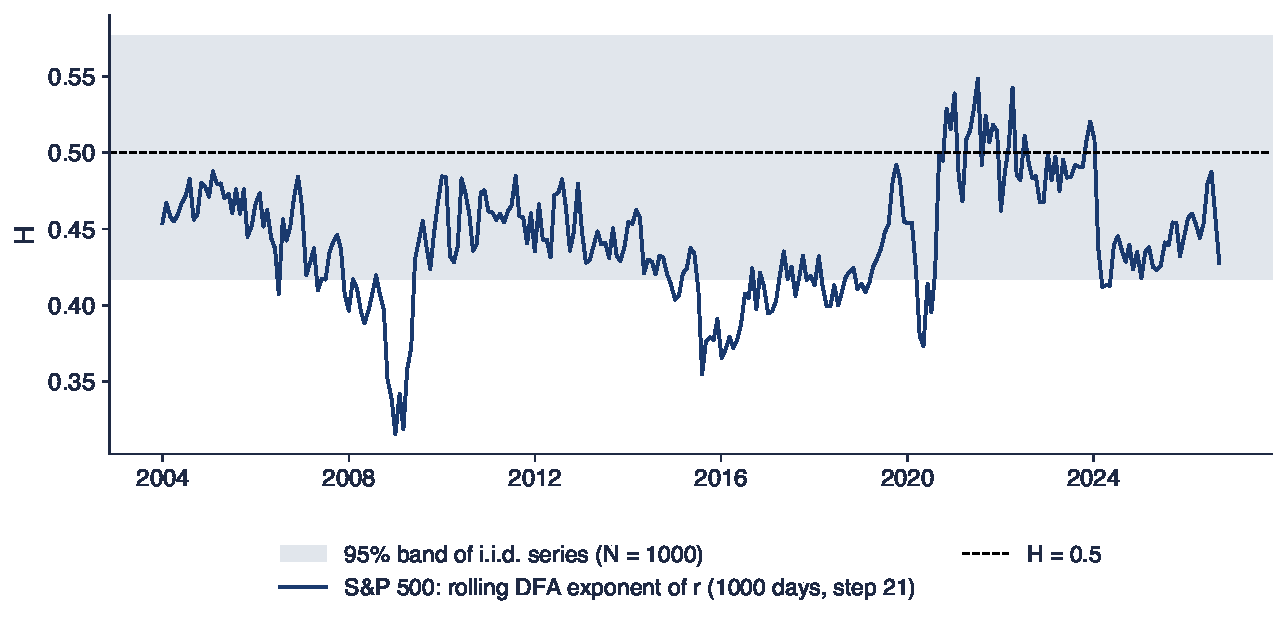
\includegraphics[width=0.96\textwidth,height=0.34\textheight,keepaspectratio]{ch11_sem_b5.pdf}
\end{center}
\vspace{-2mm}
\begin{itemize}
    \item 273 de ferestre din 29 decembrie 2003; banda $[0{,}417; 0{,}577]$; $\hat H$ mediu $= 0{,}443$
    \item Minimul $0{,}316$ (31 decembrie 2008), maximul $0{,}549$ (9 iulie 2021); 22{,}3\% dintre ferestre sub bandă, 0{,}0\% peste
    \item Interpretare: nu: din întîmplare, circa 14 dintre 273 de ferestre ies din bandă, iar ferestrele consecutive se suprapun; contează doar perioadele lungi; aici perioadele sînt sub bandă (antipersistență după 2008 și în 2016), niciodată peste
\end{itemize}\sfmquantlet{Ch_11}{SFM_ch11_seminar}
\end{frame}

\begin{frame}{B6: exponenți pe ferestre mobile pentru DAX și Banca Transilvania [Propus]}
\itemsize{\footnotesize}
\begin{itemize}
\item \textbf{Întrebarea}: se confirmă rezultatul din B5 pentru DAX și Banca Transilvania? Model: B5.
\item \textbf{Date}: DAX din 2000, TLV din 2010; randamente logaritmice zilnice în \%
\item \textbf{Cerințe}
\begin{enumerate}
    \item Estimați exponentul DFA pe ferestre mobile ca în B5.
    \item Raportați ponderea ferestrelor sub bandă și peste bandă, precum și minimul și maximul, cu datele lor.
    \item Comparați exponentul mediu din prima și din ultima treime a ferestrelor.
    \item Interpretare: care piață pare mai stabilă în timp?
\end{enumerate}
\item \textbf{Raportați}: un tabel și două fraze
\item Notebook: secțiunea B6
\end{itemize}
\end{frame}

\ifsolutions
\begin{frame}{B6: rezolvare [Propus]}
\itemsize{\footnotesize}
\begin{center}
\scriptsize
\begin{tabular}{lrrrrrr}
\toprule
 & ferestre & sub & peste & minimul & maximul & prima / ultima treime \\
\midrule
DAX & 276 & 4{,}0\% & 1{,}8\% & $0{,}391$ (20 februarie 2009) & $0{,}609$ (22 noiembrie 2021) & $0{,}462$ / $0{,}494$ \\
TLV & 133 & 2{,}3\% & 0{,}0\% & $0{,}400$ (23 iulie 2024) & $0{,}559$ (3 septembrie 2014) & $0{,}512$ / $0{,}481$ \\
\bottomrule
\end{tabular}
\end{center}
\begin{itemize}
    \item Banda pentru $N = 1000$: $[0{,}417; 0{,}577]$
    \item DAX: cîteva ferestre în afara benzii, de ambele părți, în jurul extremelor din 2009 și 2021; TLV: aproape mereu în interior
    \item Interpretare: ambele sînt aproape de 0,5 în cea mai mare parte a timpului; niciuna nu arată o abatere durabilă, spre deosebire de BET în primii ani
\end{itemize}\sfmquantlet{Ch_11}{SFM_ch11_seminar}
\end{frame}
\fi


%=============================================================================
\section{Partea C: întrebări deschise și critica unui răspuns AI}
%=============================================================================

\begin{frame}{C1: se schimbă memoria pieței în crize? [Propus]}
\itemsize{\footnotesize}
\begin{itemize}
\item \textbf{Întrebarea}: se schimbă exponentul Hurst al randamentelor sau al volatilității într-o criză, așa cum sugerează ipoteza pieței fractale?
\item \textbf{Date}: randamentele logaritmice zilnice S\&P 500 și BET; un an liniștit (2017) și doi ani de criză (septembrie 2008--august 2009, februarie 2020--februarie 2021); modele: B1, B3
\item \textbf{Cerințe}
\begin{enumerate}
    \item Estimați exponentul DFA pentru $r_t$ și $|r_t|$ și volatilitatea anualizată în fiecare dintre cei trei ani, pentru ambii indici.
    \item Calculați banda Monte Carlo pentru ferestre de circa 250 de zile.
    \item Enumerați trei motive pentru care un singur an de criză nu poate lămuri întrebarea.
    \item Interpretare: ce abordare ar separa o schimbare a memoriei de o schimbare a volatilității?
\end{enumerate}
\item \textbf{Raportați}: un tabel și un plan de proiect
\item Notebook: secțiunea C1
\end{itemize}
\end{frame}

\ifsolutions
\begin{frame}{C1: analiză de referință [Propus]}
\itemsize{\footnotesize}
\begin{center}
\scriptsize
\begin{tabular}{llrrrr}
\toprule
Indice & perioada & $N$ & DFA $r_t$ & DFA $|r_t|$ & volatilitate \\
\midrule
S\&P 500 & an liniștit 2017 & 250 & $0{,}42$ & $0{,}51$ & 6{,}7\% \\
S\&P 500 & criza 2008--2009 & 252 & $0{,}43$ & $0{,}76$ & 45{,}2\% \\
S\&P 500 & criza 2020--2021 & 251 & $0{,}69$ & $1{,}02$ & 34{,}9\% \\
BET & an liniștit 2017 & 248 & $0{,}58$ & $0{,}68$ & 10{,}5\% \\
BET & criza 2008--2009 & 249 & $0{,}44$ & $0{,}67$ & 51{,}4\% \\
BET & criza 2020--2021 & 249 & $0{,}76$ & $0{,}87$ & 25{,}2\% \\
\bottomrule
\end{tabular}
\end{center}
\begin{itemize}
    \item Banda pentru $N = 250$: $[0{,}33; 0{,}66]$; doar randamentele din 2020--2021 ale ambilor indici sînt peste ea
    \item Motive: un singur an dă o bandă largă; nivelul volatilității schimbă estimarea pentru $|r_t|$; revenirea de după martie 2020 este o tendință în interiorul ferestrei
    \item Abordare: standardizăm $r_t$ cu o volatilitate GARCH (\sfmchlink{https://danpele.github.io/SFM/RO/Cursuri/capitol9_modele_arch_garch.pdf}{Capitolul 9}) înainte de estimare; folosim multe crize și piețe, ferestre de eveniment și o bandă pe baza unui GARCH; comparăm cu abordarea wavelet din \refKrisB
\end{itemize}\sfmquantlet{Ch_11}{SFM_ch11_seminar}
\end{frame}
\fi

\begin{frame}{C2: verificați un răspuns AI [Propus]}
\itemsize{\scriptsize}
\begin{itemize}
    \item Un student a cerut unui asistent AI să interpreteze estimările memoriei lungi pentru S\&P 500 (date zilnice, din 2000). Răspunsul:
    \item \aiprompt{(a) R/S dă H = 0{,}530 pentru randamente: peste 0,5, deci randamentele au memorie lungă și tendințele pot fi exploatate.}
    \item \aiprompt{(b) H = 0{,}530 înseamnă o probabilitate de 53\% ca mîine să aibă același semn ca azi.}
    \item \aiprompt{(c) GPH dă d = 0{,}470 pentru |r|, deci H = d - 0,5 = -0{,}030: randamentele absolute sînt antipersistente.}
    \item \aiprompt{(d) Memoria lungă a lui |r| contrazice forma slabă a EMH.}
    \item \aiprompt{(e) Statistica modificată a lui Lo, V = 1{,}56, se află în [0,809; 1,862], deci memoria scurtă nu este respinsă la 5\%.}
    \item \aiprompt{(f) Pentru mai multă precizie, folosiți toate cele T/2 = 3357 de frecvențe în regresia GPH.}
    \item Cerințe
    \begin{itemize}
        \item 1. Pentru fiecare afirmație, precizați dacă este corectă; dacă nu este, formulați afirmația corectă și, acolo unde se poate, dați valoarea corectă din notebook (secțiunea C2).
        \item 2. Raportați: o listă de șase verdicte, fiecare cu un rînd de justificare.
    \end{itemize}
\end{itemize}
\end{frame}

\ifsolutions
\begin{frame}{C2: rezolvare [Propus]}
\itemsize{\footnotesize}
\begin{itemize}
    \item (a) Greșit: seriile i.i.d.\ de această lungime dau în medie R/S $0{,}544$, cu banda pînă la $0{,}575$; DFA dă $0{,}488$: nicio dovadă de memorie lungă (B1)
    \item (b) Greșit: $H$ este un exponent de scalare, nu o probabilitate
    \item (c) Greșit: $H = d + 0{,}5 = 0{,}970$: persistență puternică a volatilității
    \item (d) Greșit: forma slabă privește direcția randamentelor; volatilitatea previzibilă este compatibilă cu ea (B3, \sfmchlink{https://danpele.github.io/SFM/RO/Cursuri/capitol9_modele_arch_garch.pdf}{Capitolul 9})
    \item (e) Corect
    \item (f) Greșit: frecvențele înalte poartă dinamica de termen scurt și deplasează $\hat d$; GPH are nevoie de $m/T \to 0$; raportăm $m = T^{0{,}5}$ și $T^{0{,}6}$
\end{itemize}\sfmquantlet{Ch_11}{SFM_ch11_seminar}
\end{frame}
\fi


%=============================================================================
\section{Încheiere}
%=============================================================================

\begin{frame}{Idei de reținut}
\itemsize{\small}
\begin{itemize}
    \item R/S, DFA și GPH estimează același $H$ în moduri diferite; raportăm mai mulți estimatori, fiecare cu o bandă Monte Carlo pentru același $N$
    \item $d = H - 0{,}5$; $H$ este un exponent de scalare, nu o probabilitate
    \item Randamentele piețelor mari: fără memorie lungă; volatilitatea: memorie lungă peste tot; testul permutării o localizează în ordinea zilelor
    \item Estimările pe ferestre mobile: interpretăm perioadele lungi din afara benzii, nu ferestrele izolate
    \item Un răspuns AI este o ciornă: verificați banda, conversia dintre $d$ și $H$ și lățimea de bandă
\end{itemize}
\end{frame}

\begin{frame}{După seminar}
\itemsize{\small}
\begin{itemize}
    \item Cursul 11 dezvoltă fiecare temă de azi: FMH, autosimilaritatea, fBm și ARFIMA, estimatorii, memoria aparentă, exponenții pe ferestre mobile, scalarea riscului
    \item Încercați cerințele [Propus] în notebook; rezolvările se discută la seminar
    \item C1 poate deveni un proiect de echipă: randamente standardizate cu GARCH, multe crize, o bandă pe baza unui GARCH
    \item Lectură: \refFHH, cap.~14; \refLo; \refWeron
\end{itemize}
\end{frame}


%=============================================================================
\section{Bibliografie}
%=============================================================================

\begin{frame}{Bibliografie}
\itemsize{\tiny}
\begin{itemize}
    \item Anis, A.A., Lloyd, E.H. (1976). \href{https://doi.org/10.1093/biomet/63.1.111}{The expected value of the adjusted rescaled Hurst range of independent normal summands}. \textit{Biometrika}, 63(1), 111--116.
    \item Diebold, F.X., Inoue, A. (2001). \href{https://doi.org/10.1016/S0304-4076(01)00073-2}{Long memory and regime switching}. \textit{Journal of Econometrics}, 105(1), 131--159.
    \item Ding, Z., Granger, C.W.J., Engle, R.F. (1993). \href{https://doi.org/10.1016/0927-5398(93)90006-D}{A long memory property of stock market returns and a new model}. \textit{Journal of Empirical Finance}, 1(1), 83--106.
    \item Franke, J., Härdle, W.K., Hafner, C.M. (2019). \href{https://doi.org/10.1007/978-3-030-13751-9}{\textit{Statistics of Financial Markets: An Introduction}}, 5th ed. Springer.
    \item Geweke, J., Porter-Hudak, S. (1983). \href{https://doi.org/10.1111/j.1467-9892.1983.tb00371.x}{The estimation and application of long memory time series models}. \textit{Journal of Time Series Analysis}, 4(4), 221--238.
    \item Hosking, J.R.M. (1981). \href{https://doi.org/10.1093/biomet/68.1.165}{Fractional differencing}. \textit{Biometrika}, 68(1), 165--176.
    \item Hurst, H.E. (1951). \href{https://doi.org/10.1061/TACEAT.0006518}{Long-term storage capacity of reservoirs}. \textit{Transactions of the American Society of Civil Engineers}, 116(1), 770--799.
    \item Kristoufek, L. (2013). \href{https://doi.org/10.1038/srep02857}{Fractal markets hypothesis and the global financial crisis: wavelet power evidence}. \textit{Scientific Reports}, 3, 2857.
    \item Lo, A.W. (1991). \href{https://doi.org/10.2307/2938368}{Long-term memory in stock market prices}. \textit{Econometrica}, 59(5), 1279--1313.
    \item Mandelbrot, B.B., Van Ness, J.W. (1968). \href{https://doi.org/10.1137/1010093}{Fractional Brownian motions, fractional noises and applications}. \textit{SIAM Review}, 10(4), 422--437.
    \item Peng, C.-K., Buldyrev, S.V., Havlin, S., Simons, M., Stanley, H.E., Goldberger, A.L. (1994). \href{https://doi.org/10.1103/PhysRevE.49.1685}{Mosaic organization of DNA nucleotides}. \textit{Physical Review E}, 49(2), 1685--1689.
    \item Peters, E.E. (1994). \href{https://www.wiley.com/en-us/Fractal+Market+Analysis\%3A+Applying+Chaos+Theory+to+Investment+and+Economics-p-9780471585244}{\textit{Fractal Market Analysis: Applying Chaos Theory to Investment and Economics}}. Wiley.
    \item Weron, R. (2002). \href{https://doi.org/10.1016/S0378-4371(02)00961-5}{Estimating long-range dependence: finite sample properties and confidence intervals}. \textit{Physica A}, 312(1--2), 285--299.
\end{itemize}
\end{frame}

\end{document}
